%definira klasu dokumenta 
\documentclass[12pt]{report} 

%prostor izmedu naredbi \documentclass i \begin{document} se zove uvod. U njemu se nalaze naredbe koje se odnose na cijeli dokument

%osnovni LaTex ne može riješiti sve probleme, pa se koriste različiti paketi koji olakšavaju izradu željenog dokumenta
\usepackage[croatian]{babel} 
\usepackage{amssymb}
\usepackage{amsmath}
\usepackage{txfonts}
\usepackage{mathdots}
\usepackage{titlesec}
\usepackage{array}
\usepackage{lastpage}
\usepackage{etoolbox}
\usepackage{tabularray}
\usepackage{color, colortbl}
\usepackage{adjustbox}
\usepackage{geometry}
\usepackage[classicReIm]{kpfonts}
\usepackage{hyperref}
\usepackage{fancyhdr}
\usepackage{listings}

\usepackage{float}
\usepackage{setspace}
\restylefloat{table}


\patchcmd{\chapter}{\thispagestyle{plain}}{\thispagestyle{fancy}}{}{} %redefiniranje stila stranice u paketu fancyhdr

%oblik naslova poglavlja
\titleformat{\chapter}{\normalfont\huge\bfseries}{\thechapter.}{20pt}{\Huge}
\titlespacing{\chapter}{0pt}{0pt}{40pt}


\linespread{1.3} %razmak između redaka

\geometry{a4paper, left=1in, top=1in,}  %oblik stranice

\hypersetup{ colorlinks, citecolor=black, filecolor=black, linkcolor=black,	urlcolor=black }   %izgled poveznice


%prored smanjen između redaka u nabrajanjima i popisima
\newenvironment{packed_enum}{
	\begin{enumerate}
		\setlength{\itemsep}{0pt}
		\setlength{\parskip}{0pt}
		\setlength{\parsep}{0pt}
	}{\end{enumerate}}

\newenvironment{packed_item}{
	\begin{itemize}
		\setlength{\itemsep}{0pt}
		\setlength{\parskip}{0pt}
		\setlength{\parsep}{0pt}
	}{\end{itemize}}




%boja za privatni i udaljeni kljuc u tablicama
\definecolor{LightBlue}{rgb}{0.9,0.9,1}
\definecolor{LightGreen}{rgb}{0.9,1,0.9}

%Promjena teksta za dugačke tablice
\DefTblrTemplate{contfoot-text}{normal}{Nastavljeno na idućoj stranici}
\SetTblrTemplate{contfoot-text}{normal}
\DefTblrTemplate{conthead-text}{normal}{(Nastavljeno)}
\SetTblrTemplate{conthead-text}{normal}
\DefTblrTemplate{middlehead,lasthead}{normal}{Nastavljeno od prethodne stranice}
\SetTblrTemplate{middlehead,lasthead}{normal}

%podesavanje zaglavlja i podnožja

\pagestyle{fancy}
\lhead{Programsko inženjerstvo}
\rhead{PassDirect}
\lfoot{CozySolutions}
\cfoot{stranica \thepage/\pageref{LastPage}}
\rfoot{\today}
\renewcommand{\headrulewidth}{0.2pt}
\renewcommand{\footrulewidth}{0.2pt}


\begin{document} 
	
	
	
	\begin{titlepage}
		\begin{center}
			\vspace*{\stretch{1.0}} %u kombinaciji s ostalim \vspace naredbama definira razmak između redaka teksta
			\LARGE Programsko inženjerstvo\\
			\large Ak. god. 2021./2022.\\
			
			\vspace*{\stretch{3.0}}
			
			\huge $PassDirect$\\
			\Large Dokumentacija, Rev. \textit{$2 $}\\
			
			\vspace*{\stretch{12.0}}
			\normalsize
			Grupa: \textit{$CozySolutions$}\\
			Voditelj: \textit{Tomislav Pavković}\\
			
			
			\vspace*{\stretch{1.0}}
			Datum predaje: \textit{14.01.2021.}\\
	
			\vspace*{\stretch{4.0}}
			
			Nastavnik: \textit{Daria Primorac}\\
		
		\end{center}	

	
	\end{titlepage}

	
	\tableofcontents


	\chapter{Dnevnik promjena dokumentacije}
		
		
		\begin{longtblr}[
				label=none
			]{
				width = \textwidth, 
				colspec={|X[2]|X[13]|X[3]|X[3]|}, 
				rowhead = 1
			}
			\hline
			\textbf{Rev.}	& \textbf{Opis promjene/dodatka} & \textbf{Autori} & \textbf{Datum}\\[3pt] \hline
			0.1 & Napravljen predložak.				& Mirta Vučinić & 25.10.2021. 		\\[3pt] \hline 
			0.2 & Funkcionalni zahtjevi,UC.				& Ivan Hajpek & 28.10.2021. 		\\[3pt] \hline 
			0.3 & UC dijagram.						& Martina Galić & 28.10.2021. 		\\[3pt] \hline 
			
			0.4 & DB dijagram i sekvencijski dijagrami.		& Martina Galić & 03.11.2021. 		\\[3pt] \hline 	
			0.5 & DB dijagram.						& Ivan Hajpek & 03.11.2021. 		\\[3pt] \hline 	
			0.6 & Dorađeni UC-ovi i sekvencijski dijagrami.	& Ivan Hajpek & 04.11.2021. 		\\[3pt] \hline 
			0.7 & Dorađeni UC-ovi i dijagram baze podataka.	& Martina Galić & 04.11.2021. 		\\[3pt] \hline 
			0.8 &Napisan opis za entitete. 				& Martina Galić & 07.11.2021. 		\\[3pt] \hline 
			0.9 & Napisan kratak opis baze i pojedinih entiteta.	& Ivan Hajpek & 08.11.2021. 		\\[3pt] \hline 
			0.10 & Opis arhitekture sustava.				& Martina Galić & 10.11.2021. 		\\[3pt] \hline 
			0.11 & Opis dizajna sustava i ostali zahtjevi.		& Ivan Hajpek & 10.11.2021. 		\\[3pt] \hline 
			0.12 & Dorađeni sekv. dijagrami i pregled dokumentacije.		& Ivan Hajpek & 15.11.2021. 		\\[3pt] \hline 
			0.13 & Dorađeni sekv. dijagrami i opis projektnog zadatka.		& Martina Galić & 15.11.2021. 		\\[3pt] \hline 
			0.14 & Izmjena BP i opis Controller Diagrama.		& Ivan Hajpek & 16.11.2021. 		\\[3pt] \hline 
			0.15 & Class Diagrams.		& Martina Galić & 16.11.2021. 		\\[3pt] \hline 
			0.16 & Dodatak, literatura, opis sastanaka.		&Ivan Hajpek& 19.11.2021. 		\\[3pt] \hline 
			0.17 & Tablica aktivnosti i izmjena pojedinih dijagrama.		& Martina Galić & 19.11.2021. 		\\[3pt] \hline 
			1.1 & Dodan dijagram atkivnosti.		& Ivan Hajpek & 19.12.2021. 		\\[3pt] \hline 
			1.2 & Popravljene greške s prve predaje.		& Krešimir Pavlović & 19.12.2021. 		\\[3pt] \hline 
			1.3 & Dodan dijagram stanja.		& Krešimir Pavlović & 20.12.2021. 		\\[3pt] \hline 
			1.4 & Dodan drugi dijagram atkivnosti.		& Ivan Hajpek & 20.12.2021. 		\\[3pt] \hline 
			1.5 & Dodan opis dijagrama aktivnosti, dopunjeni ostali zahtjevi, sitne promjene ostatka.		& Ivan Hajpek & 20.12.2021. 		\\[3pt] \hline
			1.6 & Dodan opis dijagrama stanja.		& Krešimir Pavlović & 4.1.2022. 		\\[3pt] \hline
			1.7 & Dodan dijagram komponenti.		& Krešimir Pavlović & 5.1.2022. 		\\[3pt] \hline
			1.8 & Dodan dijagram razmještaja, dopunjen dnevnik sastajanja, dodan opis korištenih tehnologija, dodan zaključak.		& Ivan Hajpek & 6.1.2022. 		\\[3pt] \hline
			1.9 & Dodan opis puštanja aplikacije u pogon.		& Krešimir Pavlović & 10.1.2022. 		\\[3pt] \hline
			1.10 & Napravljen specifikacijski dijagram klasa.		& Ivan Hajpek & 10.1.2022. 		\\[3pt] \hline
			1.11 & Dodano ispitivanje sustava.		& Krešimir Pavlović & 12.1.2022. 		\\[3pt] \hline
			1.12 & Opis dijagrama klasa, dodan UC, promjena baze i dijagrama.		& Ivan Hajpek & 12.1.2022. 		\\[3pt] \hline
			1.13 & Unit testing dodan.		& Krešimir Pavlović, Ivan Hajpek & 12.1.2022. 		\\[3pt] \hline
		\end{longtblr}
	
	
		
	\chapter{Opis projektnog zadatka}
\vspace{1cm}

Velik problem sadašnjice, a i prošlosti u području željezničke strukture napokon je dobio rješenje. U prošlosti je zasigurno bilo teže riješiti problem nejednolike raspodjele mase unutar vagona vlaka zbog nedostatka naprednije tehnologije, što je uzrokovalo povećanje istrošenosti kotača, slabljenje strukture osovine te postojanje veće vjerojatnosti iskliznuća vlaka iz tračnica.
Mehaničari su  stoga periodično morali održavati sustav kotača radi njegove
rekonfiguracije i optimizacije što nekada možda i nije bilo nužno, no mehaničari nisu bili sigurni te su svakako napravili potrebno održavanje, što u nekim zemljama moraju i danas, no ne i u Nizozemskoj, jednoj od najnaprednijih država po pitanju željezničkog prometa. Utvrđivanje dijela vagona na kojem je potrebno provesti održavanje je dugotrajan i kompleksan posao.  Kako bi smanjili broj nesreća uzrokovanih nastalim problemima zbog nejednolike raspodjele mase te sačuvali infrastrukturu,odnosno produžili joj životni vijek, Nizozemci su osmislili sustav senzora Gotcha.\\
Gotcha se sastoji od senzora postavljenih duž tračnica kolosijeka na odabranim točkama.
Pri prolasku vlaka preko senzora, senzori mjere opterećenje kotača u
stvarnom vremenu. Iz vremenskog niza podataka se tada može procijeniti akumulativna
šteta na svakom kotaču i odrediti optimalan trenutak održavanja svakog vagona.\\
Uz to što će senzor zabilježiti podatke koji pomažu pri određivanju optimalnog trenutka održavanja vagona, cilj je i doći do manjeg broja popravaka odnosno održavanja. To se postiže na način da se ravnomjerno rasporedi masa u vagonu, odnosno da putnici sjede na odgovarajućim mjestima. Dakle, postiže se pomoć u prevenciji
oštećenja nastalim nejednolikom raspodjelom mase, smanjuje se trošak održavanja i
povećava vrijeme dostupnosti vagona. Ideja aplikacije PassDirect je upućivanje putnika u odgovarajuće vagone (i perone na kojima ih mogu čekati) u svrhu optimalne distribucije njihove težine, uporabom podataka sustava senzora Gotcha. Vlakovi nad kojima se provode mjerenja namijenjeni su brzom povezivanju prigradskih naselja te nemaju omogućenu rezervaciju sjedala.\\

\textbf{Sustav senzora:}\\
Svako mjerenje senzora daje podatak koji se sastoji od: položaja senzora na pruzi, identifikacijske oznake vlaka, brzine vlaka, vrijeme mjerenja te niza prirodnih brojeva, po dva za svaki vagon. Niz prirodnih brojeva označava višak detektirane mase u kilogramima u svakom vagonu i to jedan podatak za prednji dio vagona, a drugi za stražnji dio. Na primjer:  80, 60, 110, 220, 756 i 923. Prvi vagon (80,60) je uravnotežen, drugi vagon (110, 220) također, dok treći vagon (756, 923) ima najviše putnika no i najveću razliku između prednjeg i stražnjeg dijela. Sva mjerenja na pojedinačnom vlaku obavljaju su istovremeno. Zanemarujemo razliku između lijeve i desne strane vagona. PassDirect je implementiran kao web aplikacija te podržava rad više korisnika u stvarnom vremenu.\\

Simulacija senzora ostvarena je korištenjem sustava Posthook koji šalje http zahtjeve na backend naše aplikacije s očitanjima senzora koja sadrže broj osoba na svakoj poziciji (naprijed i nazad) za svaki vagon tog vlaka.\\
Mjerenja su napisana za 3 vlaka na 3 stanice i različita su za 3 uzastopna dana te se nakon toga ponavljaju.
Vlak polazi sa stanice u Zagrebu pa prvo očitanje primamo nakon napuštanja te stanice što znači da korisnici koji kupuju kartu iz Zagreba ne dobivaju upute gdje trebaju sjesti nego imaju slobodan izbor jer je vlak prazan. Korisnici koji polaze sa sljedeće stanice (Split), nakon što vlak napusti stanicu u Zagrebu, dobivaju preporuku o broju vagona i perona te poziciji u vagonu (naprijed ili nazad) gdje trebaju sjesti. \\

Broj vagona i pozicija računaju se na temelju očitanja s prethodne stanice na sljedeći način: 
\begin{itemize}
\item Ako je razlika u broju putnika naprijed i nazad u nekom vagonu veća od 30, putnik se šalje u taj vagon (s najvećom razlikom ako ih je više takvih) na poziciju koja je manje popunjena. 
\item Ako ni u jednom vagonu razlika broja ljudi nije veća od 30, putnik se šalje u vagon s najmanjim brojem ljudi, na manje popunjenu poziciju. 
\item Ako je putnik usmjeren, podaci o broju putnika u tom vagonu se ažuriraju kako ne bi svi putnici bili usmjereni na istu poziciju.
Nakon kupnje karte, putnik prima email s kartom, a nakon što vlak napusti prethodnu stanicu, putnik prima email s ažuriranom kartom s podacima o broju vagona, perona i poziciji na koju treba sjesti. 
\item Ako korisnik kupi kartu za vlak koji je već napustio prethodnu stanicu, odmah prima email s kartom koja sadrži podatke o broju vagona, perona i poziciji na koju treba sjesti kako bi izbjegli nepotrebno slanje više emailova.\\
\end{itemize}
Ako vlak kasni na određenu stanicu (senzor) više od dvije minute, na početnoj stranici aplikacije, kod pregleda voznog reda na toj i svim sljedećim stanicama, vrijeme dolaska postaje crveno kako bi se naglasilo da vlak kasni i vjerojatno neće stići u to vrijeme. Čak i kada vlak dođe na tu stanicu (senzor), ako je vrijeme kada je trebao doći prošlo za više od 2 minute, na sljedećim stanicama ostaje oznaka kašnjenja. Ako vlak to kašnjenje nadoknadi te na sljedeću stanicu dođe na vrijeme, oznaka kašnjenja se miče za sljedeće stanice.\\

    \textbf{Korisnik može imati ulogu:}
    \begin{itemize}
    \item Administratora 
    \item Konkretnog korisnika\\
    \end{itemize}
    
    \underline{Administrator} može pregledati i ukloniti korisnike te pregledati njihove transakcije, no nije zadužen za mijenjanje voznog reda. Također ima pristup svim provedenim transakcijama, bazi podataka korisnika i redu vožnje. PassDirect upravlja rasporedom putnika dok je za vozni red zadužen drugi ogranak željeznice. \\
    
    \underline{Konkretan korisnik} može pristupiti funkcionalnostima web stranice PassDirect registracijom, odnosno kreiranjem svog korisničkog računa te prijavom na isti.\\ Prilikom registracije, korisnik unosi svoje podatke, i to:
    \begin{itemize}
        \item ime
        \item prezime 
        \item e-mail adresu 
        \item lozinku\\
    \end{itemize} 
    
 

\textbf{Nakon prijave i registracije:}\\
Nakon uspješne registracije i prijave, korisniku se na pregledniku prikazuju ponuđena stajališta, od kojih on može odabrati jedno. Odabir ga vodi na listu dolazećih vlakova na to stajalište (u stvarnom vremenu). Informacije koje korisnik treba dobiti odabirom stajališta su: 
\begin{itemize}
    \item identifikacijska oznaka vlaka
    \item krajnje odredište
    \item vrijeme dolaska\\
\end{itemize}
Zadnje tri informacije bi trebale biti istaknute i dane samo za one vlakove koji su napustili prethodno stajalište.  Do zaključka je li vlak napustio prethodno stajalište dolazimo uporabom senzora koji se nalazi na prošlom stajalištu. Ako je mjerenje detektirano, vlak je napustio prethodno stajalište. Vlak se zadržava na svakom stajalištu 10 minuta. Vrijeme u kojem senzor detektira vlak, koristimo za određivanje kašnjenja vlaka na sljedeće stajalište, točnije određujemo hoće li kasniti i koliko će kasniti.\\



\textbf{Klasično pretraživanje voznog reda:}\\
Klasično pretraživanje uključuje:
\begin{itemize}
    \item odabir mjesta polaska
    \item odabir mjesta dolaska
    \item datum\\
\end{itemize}
Na zaslonu se potom  izlistavaju odgovarajuće linije vlakova zajedno s ostalim informacijama (npr. identifikacijska oznaka vlaka, mjesto i vrijeme polaska, mjesto i vrijeme dolaska, kolosijek dolaska, kašnjenje vlaka i cijena karte). \\

\textbf{Kupovina karte:}\\
Skup korisnika zainteresiranih za konzumaciju prijevozne usluge, prilikom prikazivanja linija, mogu kupiti kartu za svaku od njih. PassDirect sadrži upitnik koji oponaša plaćanje. Pri prvoj transakciji, korisnik popunjava formular, no pri svakoj narednoj, formular se popunjava sam. Nakon kupovine, korisniku stižu dva e-maila. U jednom e-mailu se nalazi kupljena karta, a u drugom obavijest koja ga upućuje na određeni kolosijek i peron koji je procijenjen kao najpogodniji. Drugi e-mail treba stići tek nakon što vlak napusti prethodno stajalište.
Drugi e-mail treba sadržavati:
\begin{itemize}
    \item informativni tekst
    \item šifru vlaka
    \item vrijeme njegovog dolaska
    \item kolosijek
    \item uputu za korisnika o prikladnom vagonu
    \item dijelu vagona 
    \item broju perona\\
\end{itemize} 
Naravno, cilj aplikacije jest uputiti putnika u prazniji dio najmanje okupiranog vagona.\\




\textbf{Slična programska rješenja:}\\
Postoje mnoga slična programska rješenja koja omogućavaju korisniku kupovinu karte, odabir početnog i krajnjeg stajališta koji rezultira izlistavanjem svih linija. Jedna od njih je naravno HŽPP-ova stranica. Navedena stranica ima implementirane sve funkcionalnosti kao i PassDirect poput kupovine karte, pregleda svih linija, pregleda svih linija s obzirom na početno i krajnje stajalište, datum, vrijeme i slično, no s obzirom da u Hrvatskoj još nije u primjenu stupio Gotcha sustav senzora, na ovako napredno rješenje kao u Nizozemskoj ćemo morati sačekati. 
\begin{figure}[H]
					\centering
					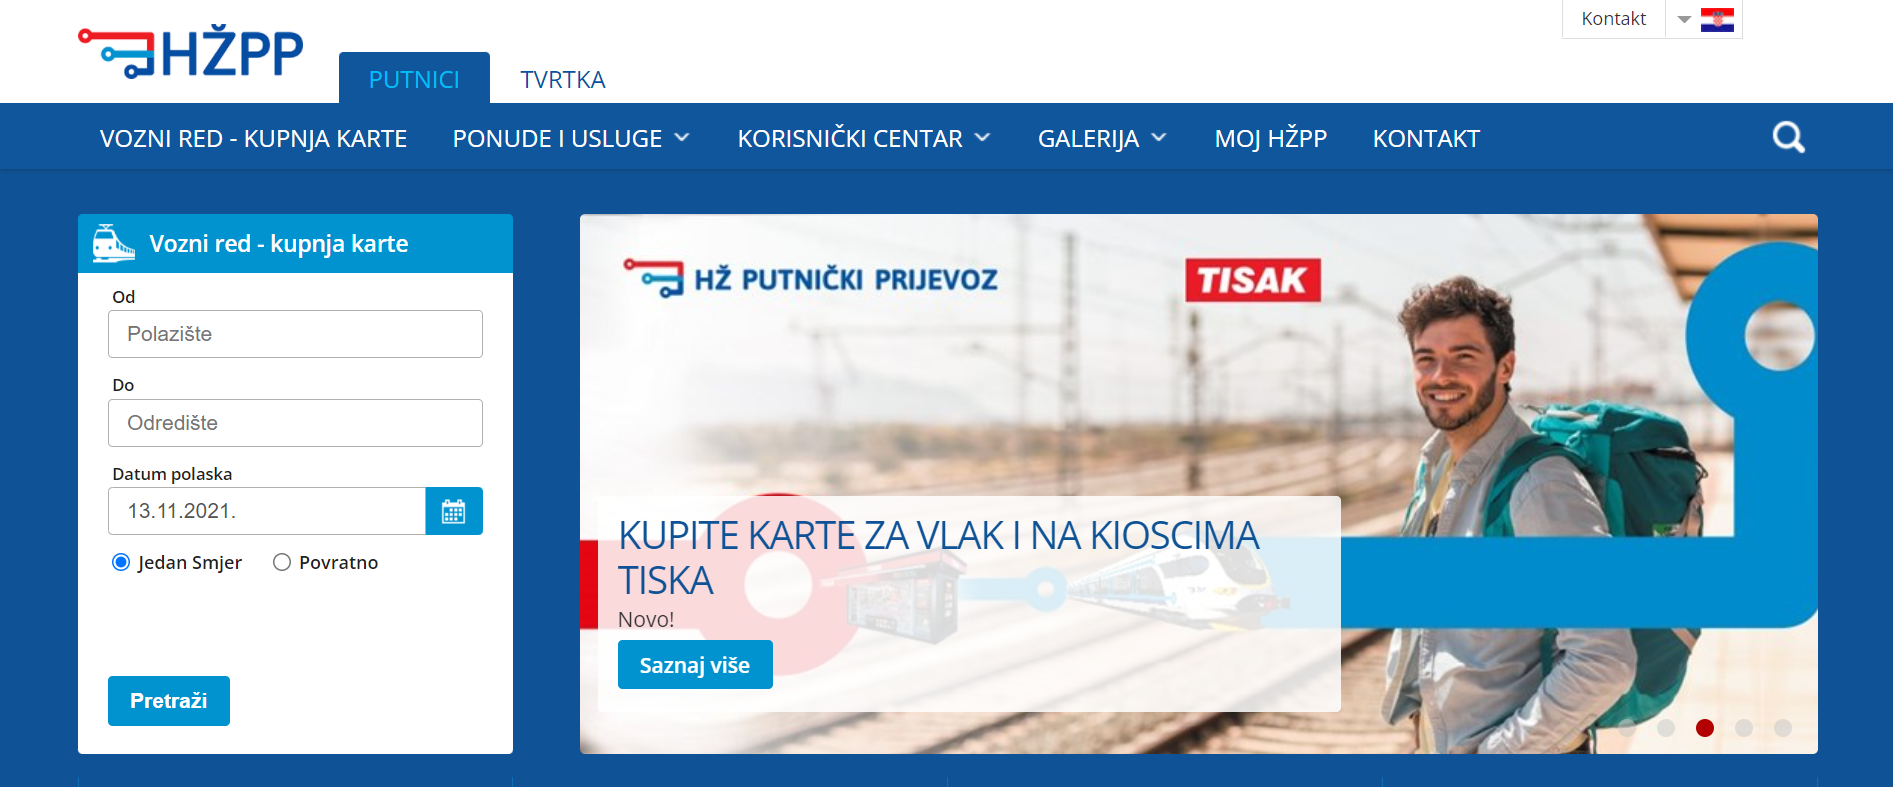
\includegraphics[width=1\linewidth]{"slike/hzpp.png"}
					\caption{Web stranica HŽPP-a}
					\label{fig:hzpp}
				\end{figure}
Također je tu i web aplikacija CityMapper koja sugerira korisniku mjesto sjedenja, no ne s obzirom na Gotcha sustav, nego s obzirom na korisnikove potrebe. Konkretnije, predlaže najbolje mjesto s obzirom na korisnikovo krajnje stajalište ili presjedanje. CityMapper posjeduje sve navedene funkcionalnosti kao i HŽPP web stranica.
 No, jako je malo web aplikacija koje sugeriraju korisniku koje mjesto bi bilo poželjno koristiti. 
 \begin{figure}[H]
					\centering
					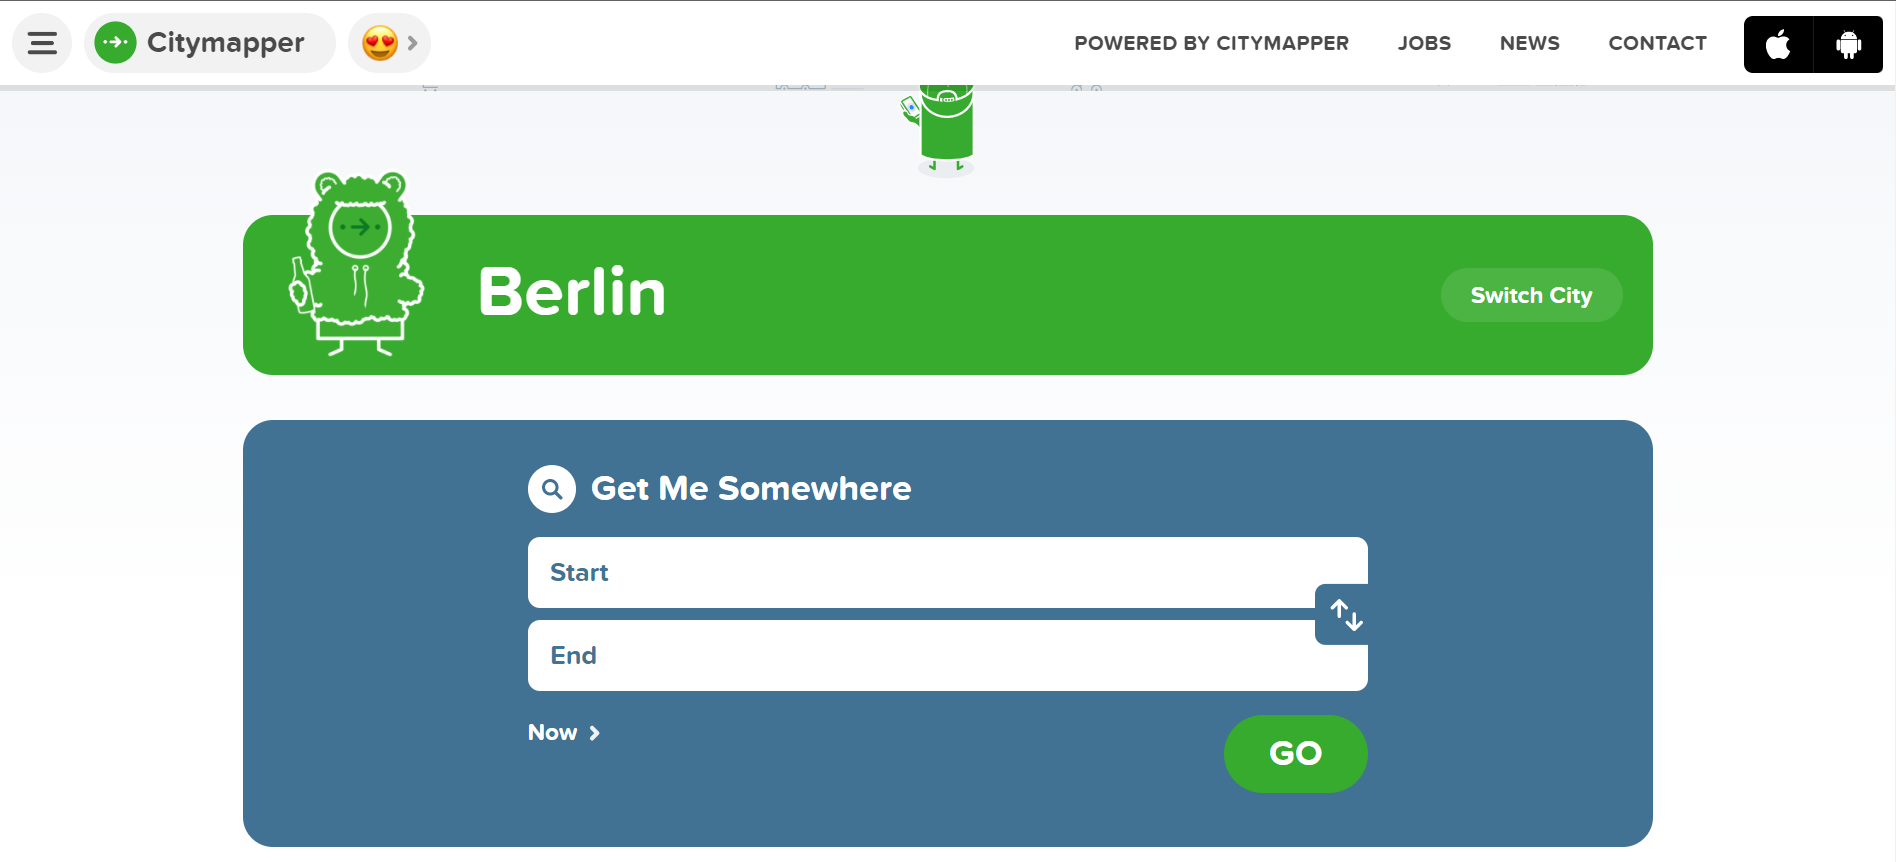
\includegraphics[width=1\linewidth]{"slike/cityMapper.png"}
					\caption{Web stranica cityMapper}
					\label{fig:cityMapper}
				\end{figure}


\textbf{Moguća nadogradnja:}\\
\begin{itemize}
    \item Web aplikaciju PassDirect bi se moglo unaprijediti dodavanjem novih funkcionalnosti poput zaključivanja o potrebi obnove infrastrukture na osnovu mjerenja senzora. Predviđanjem obnove, mogli bismo pravovremeno ukloniti određene vozne redove kako korisnik ne bi dobivao krivu informaciju pri ranoj kupovini karte ili ako dođe do otkazivanja linije, aplikacija bi trebala poslati e-mail korisniku.
    Uz to bi bila poželjna i funkcionalnost koja bi pri određivanju sjedala za korisnika, uz podatke mjerenja, uzimala u obzir i krajnje stajalište korisnika ili presjedanje i na taj način poticala korisnika još više da koristi upravo to određeno sjedalo, jer u tom slučaju, korist bi imao i korisnik i željeznički prijevoz. 
    \item Aplikaciju je moguće proširiti i na mobilnu platformu čime bi njena funkcionalnost bila fleksibilnija. Korisnik bi umjesto korištenja e-maila imao opciju čuvanja karte te dohvaćanja informacija o narednoj vožnji nakon kupovine na samoj mobilnoj aplikaciji. Također, bila bi olakšana komunikacija s korisnikom u slučaju promjena u redu vožnje (npr. promjena perona ili otkazivanja vožnje) putem notifikacija.
\end{itemize}




	\chapter{Specifikacija programske potpore}
		
	\section{Funkcionalni zahtjevi}
			
			\noindent \textbf{Dionici:}
			
			\begin{packed_enum}
				
				\item Klijent
				\item Administrator				
				\item Razvojni tim
				\item Željezničko poduzeće
				
			\end{packed_enum}
			
			\noindent \textbf{Aktori i njihovi funkcionalni zahtjevi:}
			
			
			\begin{packed_enum}
				\item  \underbar{Neregistrirani korisnik (inicijator) može:}
				
				\begin{packed_enum}
					
					\item se registrirati kako bi se mogao prijaviti u aplikaciju
					
				\end{packed_enum}
			
				\item  \underbar{Klijent (inicijator) može:}
				
				\begin{packed_enum}
					
					\item se prijaviti u stranicu kako bi mogao koristiti aplikaciju
					\item odabrati jedno od ponuđenih stajališta vlaka i dobiti prikaz informacija za svaku ponuđenu vožnju (identifikacijsku oznaku vlaka, krajnje odredište i vrijeme dolaska)
					\item klasično pretražiti red
vožnje u bilo kojem trenutku(odabir mjesta polaska, odabir mjesta dolaska i datum)
					\item kupiti kartu za svaku prikazanu liniju na aplikaciji
					\item obrisati profil/račun
					
				\end{packed_enum}
				
				\item  \underbar{Administrator (inicijator) može:}
				
				\begin{packed_enum}
					
					\item pristupati podatcima o klijentima te pregledati njihove transakcije
					\item pristupati redu vožnje
					\item brisati klijente
					
				\end{packed_enum}				
				
				\item  \underbar{Aplikacija (sudionik) mora:}
				
				\begin{packed_enum}
					
					\item poslati mail s kupljenom kartom klijentu nakon što je klijent plati
					\item poslati drugi mail kojim ga upućuje na određeni kolosijek i peron
					
				\end{packed_enum}
				
				\item  \underbar{Baza podataka (sudionik):}
				
				\begin{packed_enum}
					
					\item pohranjuje podatke o korisnicima i svim njihovim provedenim transakcijama(kupljenim kartama)
					\item pohranjuje podatke o voznom redu, poput polaznog i krajnjeg stajališta, cijene karte, datuma linije i slično
					
				\end{packed_enum}
				
			\end{packed_enum}
			
			\eject 
			
			
				
			\subsection{Obrasci uporabe}
				
				\subsubsection{Opis obrazaca uporabe}

					\noindent \underbar{\textbf{UC1 - Registracija}}
					\begin{packed_item}
	
						\item \textbf{Glavni sudionik: } Korisnik
						\item  \textbf{Cilj:} Stvaranje korisničkog računa za prijavu u sustav
						\item  \textbf{Sudionici:} Baza podataka
						\item  \textbf{Preduvjet:} --
						\item  \textbf{Opis osnovnog tijeka:}
						
						\item[] \begin{packed_enum}
	
							\item Korisnik odabire opciju registracije
							\item Korisnik upisuje potrebne vlastite podatke
							\item Korisnik potvrđuje registraciju
							\item Sustav validira podatke i sprema ih u bazu podataka u slučaju ispravnosti 
							
						\end{packed_enum}
						
						\item  \textbf{Opis mogućih odstupanja:}
						
						\item[] \begin{packed_item}
	
							\item[2.a] Odabir već postojećeg korisničkog imena, odnosno e-maila, upis korisničkog podatka u nedozvoljenom formatu ili pružanje neispravnog formata e-maila
							\item[] \begin{packed_enum}
								
								\item Sustav obavijesti korisnika o neuspješnom upisu podatka i vraća ga na stranicu za registraciju
								\item Korisnik mijenja pogrešne podatke ili odustaje od registracije
								
							\end{packed_enum}
							
						\end{packed_item}
					\end{packed_item}
					
					\noindent \underbar{\textbf{UC2 - Prijava}}
					\begin{packed_item}
	
						\item \textbf{Glavni sudionik: } Klijent, administrator
						\item  \textbf{Cilj:} Prijava za pristup aplikaciji za kupnju karata
						\item  \textbf{Sudionici:} Baza podataka
						\item  \textbf{Preduvjet:} Registracija
						\item  \textbf{Opis osnovnog tijeka:}
						
						\item[] \begin{packed_enum}
	
							\item Korisnik unosi korisničko ime i lozinku
							\item Korisnik potvrđuje navedene podatke
							\item Korisnik dobiva pristup aplikaciji
							
						\end{packed_enum}
						
						\item  \textbf{Opis mogućih odstupanja:}
						
						\item[] \begin{packed_item}
	
							\item[2.a] Neispravno korisničko ime ili lozinka
							\item[] \begin{packed_enum}
								
								\item Sustav obavijesti korisnika o neuspješnoj prijavi i vrati ga na stranicu za prijavu 
								
							\end{packed_enum}
							
						\end{packed_item}
					\end{packed_item}
					
					\noindent \underbar{\textbf{UC3 - Pregled vlakova za stajalište}}
					\begin{packed_item}
	
						\item \textbf{Glavni sudionik: } Klijent
						\item  \textbf{Cilj:} Pregledati sve dolazeće vlakove na stajalište koje je klijent odabrao
						\item  \textbf{Sudionici:} Baza podataka
						\item  \textbf{Preduvjet:} Prijava
						\item  \textbf{Opis osnovnog tijeka:}
						
						\item[] \begin{packed_enum}
	
							\item Korisnik odabire stajalište koje mu treba
							\item Korisnik potvrđuje odabir
							\item Aplikacija prikazuje popis dolazećih vlakova na odabrano stajalište
							
						\end{packed_enum}
						
						\item  \textbf{Opis mogućih odstupanja:}
						
						\item[] \begin{packed_item}
	
							\item[2.a] Korisnik nije odabrao stajalište
							\item[] \begin{packed_enum}
								
								\item Sustav obavijesti korisnika o neuspješnom zahtjevu i zatraži odabir stajališta
								
							\end{packed_enum}
							
						\end{packed_item}
					\end{packed_item}
					
					\noindent \underbar{\textbf{UC4 - Pretraživanje voznog reda}}
					\begin{packed_item}
	
						\item \textbf{Glavni sudionik: } Klijent
						\item  \textbf{Cilj:} Pretražiti vozni red
						\item  \textbf{Sudionici:} Baza podataka
						\item  \textbf{Preduvjet:} Prijava
						\item  \textbf{Opis osnovnog tijeka:}
						
						\item[] \begin{packed_enum}
	
							\item Korisnik odabire mjesto polaska i dolaska
							\item Korisnik odabire željeni datum
							\item Korisnik potvrđuje odabir
							\item Aplikacija prikazuje vozni red za odabrane podatke
							
						\end{packed_enum}
						
						\item  \textbf{Opis mogućih odstupanja:}
						
						\item[] \begin{packed_item}
	
							\item[3.a] Korisnik nije odabrao mjesto polaska, dolaska ili datum
							\item[] \begin{packed_enum}
								
								\item Sustav obavijesti korisnika o neuspješnom zahtjevu i zatraži ponovni odabir i unos
								
							\end{packed_enum}
							
						\end{packed_item}
					\end{packed_item}
					
					\noindent \underbar{\textbf{UC5 - Kupnja karte}}
					\begin{packed_item}
	
						\item \textbf{Glavni sudionik: } Klijent
						\item  \textbf{Cilj:} Kupiti kartu za vlak
						\item  \textbf{Sudionici:} Baza podataka
						\item  \textbf{Preduvjet:} Prijava i pretraga
						\item  \textbf{Opis osnovnog tijeka:}
						
						\item[] \begin{packed_enum}
	
							\item Korisnik odabire vlak za koji želi kupiti kartu
							\item Korisnik upisuje potrebne osobne podatke za kupnju(ime, prezime, podaci o kartici itd.) ili se automatski popunjavaju ako su već upamćeni
							\item Korisnik potvrđuje kupnju
							\item Stizanje 2 e-mailova
							
						\end{packed_enum}
						
						\item  \textbf{Opis mogućih odstupanja:}
						
						\item[] \begin{packed_item}
	
							\item[2.a] Korisnik nije dobro upisao neki podatak
							\item[] \begin{packed_enum}
								
								\item Sustav obavijesti korisnika o neuspješnoj kupnji zbog neispravno unesenih podataka
								\item Korisnik ima mogućnost ponovno unijeti podatke ili odustati od kupnje
								
							\end{packed_enum}
							
						\end{packed_item}
					\end{packed_item}	
					
					\noindent \underbar{\textbf{UC6 - Pregled klijenata}}
					\begin{packed_item}
	
						\item \textbf{Glavni sudionik: } Administrator
						\item  \textbf{Cilj:} Pristupiti i pregledati podatke klijenata
						\item  \textbf{Sudionici:} Baza podataka
						\item  \textbf{Preduvjet:} Korisnik mora biti prijavljen i registriran s dodijeljenim pravom administratora
						\item  \textbf{Opis osnovnog tijeka:}
						
						\item[] \begin{packed_enum}
	
							\item Administrator odabere opciju pregledavanja klijenata
							\item Na aplikaciji se izlistaju podatci svakog korisnika aplikacije
							
						\end{packed_enum}
						
					\end{packed_item}	
					
					\noindent \underbar{\textbf{UC7 - Pregled transakcija}}
					\begin{packed_item}
	
						\item \textbf{Glavni sudionik: } Administrator
						\item  \textbf{Cilj:} Pristupiti i pregledati podatke o provedenim transakcijama
						\item  \textbf{Sudionici:} Baza podataka
						\item  \textbf{Preduvjet:} Korisnik mora biti prijavljen i registriran s dodijeljenim pravom administratora
						\item  \textbf{Opis osnovnog tijeka:}
						
						\item[] \begin{packed_enum}
	
							\item Administrator odabere opciju pregledavanja transakcija
							\item Na aplikaciji se izlistaju podatci svake provedene transakcije kroz aplikaciju
							
						\end{packed_enum}
						
					\end{packed_item}	
					
					\noindent \underbar{\textbf{UC8 - Pregled reda vožnje}}
					\begin{packed_item}
	
						\item \textbf{Glavni sudionik: } Administrator
						\item  \textbf{Cilj:} Pristupiti i pregledati vozni red
						\item  \textbf{Sudionici:} Baza podataka
						\item  \textbf{Preduvjet:} Korisnik mora biti prijavljen i registriran s dodijeljenim pravom administratora
						\item  \textbf{Opis osnovnog tijeka:}
						
						\item[] \begin{packed_enum}
	
							\item Administrator odabere opciju pregledavanja voznog reda
							\item Na aplikaciji se izlista vozni red
							
						\end{packed_enum}
						
					\end{packed_item}

					\noindent \underbar{\textbf{UC9 - Brisanje klijenta}}
					\begin{packed_item}
	
						\item \textbf{Glavni sudionik: } Administrator
						\item  \textbf{Cilj:} Obrisati odabrane korisnike
						\item  \textbf{Sudionici:} Baza podataka
						\item  \textbf{Preduvjet:} Korisnik mora biti prijavljen i registriran s dodijeljenim pravom administratora
						\item  \textbf{Opis osnovnog tijeka:}
						
						\item[] \begin{packed_enum}
	
							\item Administrator odabere klijenta na listi klijenata
							\item Administrator obriše odabranog klijenta opcijom brisanja te potvrdom odluke
							\item Aplikacija ga vraća na osvježenu listu klijenata
							
						\end{packed_enum}
						
					\end{packed_item}	
					
					
						\noindent \underbar{\textbf{UC10 - Odjava}}
					\begin{packed_item}
	
						\item \textbf{Glavni sudionik: } Klijent
						\item  \textbf{Cilj:} Odjaviti se
						\item  \textbf{Sudionici:} 
						\item  \textbf{Preduvjet:} Korisnik mora biti registriran i prijavljen 
						\item  \textbf{Opis osnovnog tijeka:}
						
						\item[] \begin{packed_enum}
	
							\item Klijent zatraži odjavu
							\item Klijentu je obrisana sesija
							\item Klijent je poslan na stranicu za prijavu
							
							
						\end{packed_enum}
						
					\end{packed_item}

					\noindent \underbar{\textbf{UC11 - Brisanje računa}}
					\begin{packed_item}
	
						\item \textbf{Glavni sudionik: } Klijent
						\item  \textbf{Cilj:} Obrisati račun na PassDirect stranici
						\item  \textbf{Sudionici:} Baza podataka
						\item  \textbf{Preduvjet:} Korisnik mora biti prijavljen i registiran
						\item  \textbf{Opis osnovnog tijeka:}
						
						\item[] \begin{packed_enum}
	
							\item Klijent odabire dugme s opcijom brisanja računa na PassDirect stranici
							\item Klijentu se izbaci obavijest s potvrdom brisanja računa, gdje bira između potvrde i odustajanja
							\item Klijent bira opciju
							\item Aplikacija ostane na istoj stranici ako odustane, a ukoliko potvrdi, vraća ga na Login stranicu 
							
						\end{packed_enum}
						
					\end{packed_item}
					
				\subsubsection{Dijagrami obrazaca uporabe}
				
		
		\begin{figure}[H]
			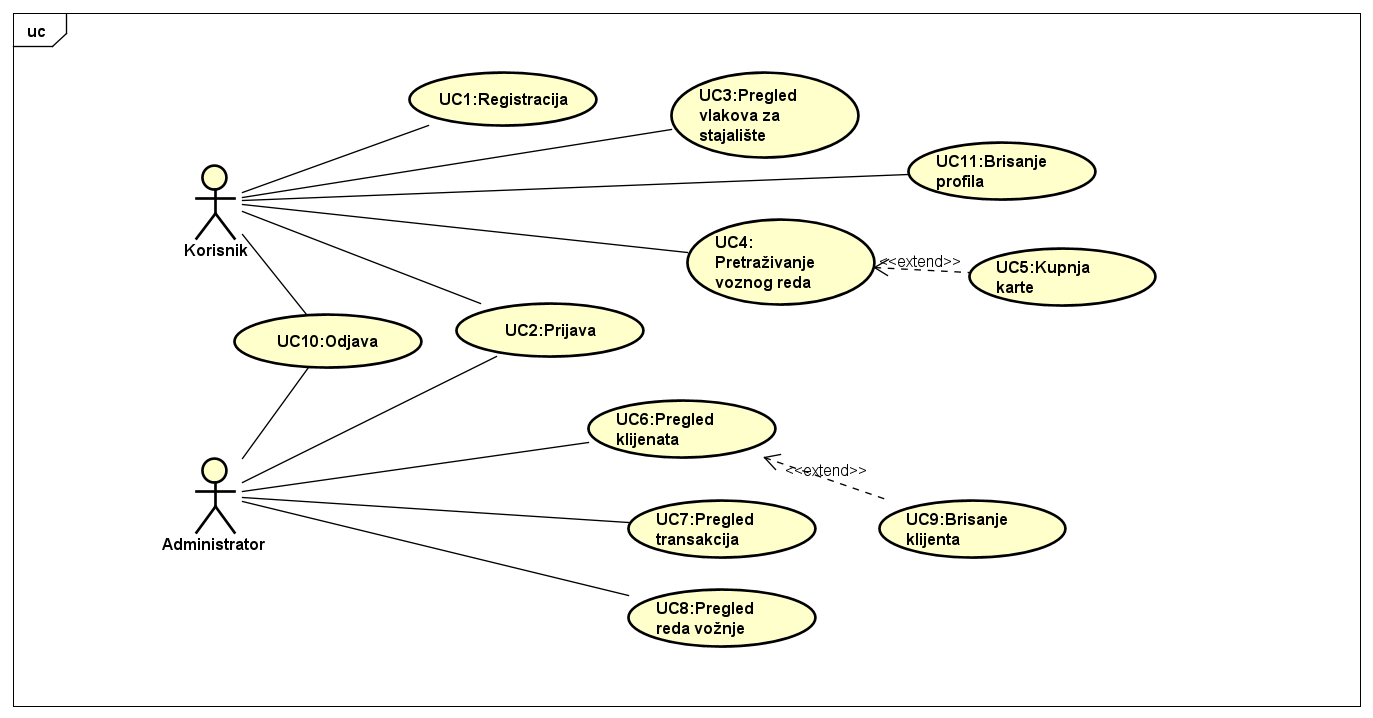
\includegraphics[width=\textwidth]{slike/UCdiagram.PNG} %veličina u odnosu na širinu linije
			\caption{UC dijagram}
			\label{fig:promjene1} %label mora biti drugaciji za svaku sliku
		\end{figure}
				\eject
	
					
				\eject		
				
			\subsection{Sekvencijski dijagrami}

				\noindent \underbar{\textbf{UC3 - Pregled vlakova za stajalište}}\\
				{Klijent odabire i potvrđuje stajalište za koje želi dobiti nadolazeće vlakove. Poslužitelj dohvaća i prikazuje popis i informacije o vlakovima koji stižu na odabrano stajalište.}\\
				
				% TODO: \usepackage{graphicx} required
				\begin{figure}[H]
					\centering
					\includegraphics[width=1\linewidth]{"slike/UC3-sekvencijski"}
					\caption{UC3 - Pregled vlakova za stajalište}
					\label{fig:UC3-pregled-vlakova}
				\end{figure}
		
				\noindent \underbar{\textbf{UC4 - Pretraživanje voznog reda}}\\
				{Klijent odabire mjesto polaska i dolaska te datum polaska, a poslužitelj mu vraća listu mogućih linija za unesene podatke.}\\
				
				% TODO: \usepackage{graphicx} required
				\begin{figure}[H]
					\centering
					\includegraphics[width=1\linewidth]{"slike/UC4-sekvencijski"}
					\caption{UC4 - Pretraživanje voznog reda}
					\label{fig:UC4-pregled-voznog-reda}
				\end{figure}		

				\noindent \underbar{\textbf{UC5 - Kupnja karte}}\\
				{Klijent odabire vlak za koji želi kupiti kartu pa ga poslužitelj odvede na stranicu za checkout. Ovdje unosi sve potrebne podatke za provesti transakciju, nakon čega potvrdi kupnju. Ukoliko su neki podaci netočni ili neispunjeni, poslužitelj daje ponovno mogućnost checkout-a ili odustajanje od kupnje. Kada su podaci točni i ispunjeni, klijentu se javlja uspješna kupnja.}\\
				
				% TODO: \usepackage{graphicx} required
				\begin{figure}[H]
					\centering
					\includegraphics[width=1\linewidth]{"slike/UC5-sekvencijski"}
					\caption{UC5 - Kupnja karte}
					\label{fig:UC5-kupnja-karte}
				\end{figure}	

				\noindent \underbar{\textbf{UC6 - Pregled klijenata}}\\
				{Administrator odabire opciju pregleda podataka o svim klijentima. Poslužitelj dohvaća i prikazuje popis i informacije o klijentima.}\\
				
				% TODO: \usepackage{graphicx} required
				\begin{figure}[H]
					\centering
					\includegraphics[width=1\linewidth]{"slike/UC6-sekvencijski"}
					\caption{UC6 - Pregled klijenata}
					\label{fig:UC-pregled-klijenata}
				\end{figure}

				\noindent \underbar{\textbf{UC7 - Pregled transakcija}}\\
				{Administrator odabire opciju pregleda podataka o svim provedenim transakcijama. Poslužitelj dohvaća i prikazuje popis i informacije o svim provedenim kupnjama karata.}\\
				
				% TODO: \usepackage{graphicx} required
				\begin{figure}[H]
					\centering
					\includegraphics[width=1\linewidth]{"slike/UC7-sekvencijski"}
					\caption{UC7 - Pregled transakcija}
					\label{fig:UC-pregled-transakcija}
				\end{figure}

				\noindent \underbar{\textbf{UC8 - Pregled reda vožnje}}\\
				{Administrator odabire opciju pregleda podataka o voznom redu, odnosno linijama vlakova. Poslužitelj dohvaća i prikazuje popis i informacije o svim voznim linijama vlakova.}\\
				
				% TODO: \usepackage{graphicx} required
				\begin{figure}[H]
					\centering
					\includegraphics[width=1\linewidth]{"slike/UC8-sekvencijski"}
					\caption{UC8 - Pregled voznog reda}
					\label{fig:UC-pregled-voznog-reda}
				\end{figure}

				\noindent \underbar{\textbf{UC9 - Brisanje klijenta}}\\
				{Administrator odabire klijenta te mu se izbacuje opcija za brisanje odabranog klijenta. Nakon odabira opcije, poslužitelj briše klijenta i vraća administratora na osvježenu listu klijenata.}\\
				
				% TODO: \usepackage{graphicx} required
				\begin{figure}[H]
					\centering
					\includegraphics[width=1\linewidth]{"slike/UC9-sekvencijski"}
					\caption{UC9 - Brisanje klijenta}
					\label{fig:UC-brisanje-klijenta}
				\end{figure}

				\noindent \underbar{\textbf{UC11 - Brisanje računa}}\\
				{Klijent odabire opciju brisanja računa u zaglavlju stranice. Web-aplikacija mu izbaci notifikaciju s upitom o potvrdi brisanja računa. Ukoliko klijent potvrdi, aplikacija ga vrati na Login stranicu, a u slučaju da odustane od brisanja računa, ostane na stranici na kojoj je bio. }\\
				
				% TODO: \usepackage{graphicx} required
				\begin{figure}[H]
					\centering
					\includegraphics[width=1\linewidth]{"slike/UC11-sekvencijski"}
					\caption{UC11 - Brisanje računa}
					\label{fig:UC-brisanje-racuna}
				\end{figure}
				
				
		\section{Ostali zahtjevi}
		
			\begin{packed_item}
				\item {Sustav treba omogućiti rad više korisnika u isto vrijeme.}
				\item {Sustav mora biti izveden kao web aplikacija s objektno orijentiranim jezikom.}
				\item {Komunikacija između korisnika i sustava mora biti brza i jednostavna.}
				\item {Aplikacija mora prikazivati aktualne, odnosno ažurirane podatke u svakom trenutku.}
				\item {Aplikacija mora raditi u stvarnom vremenu.}
				\item {Sustav kao valutu koristi HRK.}
				\item{Baza podataka treba biti brza, učinkovita i dobro povezana sa sustavom, otporna na bilo kakve greške korisnika i administratora.}
				\item {U slučaju pogrešaka ili zlonamjernih unosa od strane korisnika, sustav mora izbaciti odgovarajuće upozorenje}
					\begin{packed_item}
					\item {U slučaju lozinke kraće od 6 znakova, izbaci se obavijest da je nužno barem 6 znakova.}
					\item {Ukoliko neki od podataka koji se moraju ispuniti nisu ispunjeni, izbaci se upozorenje o tome.}
					\item {Prilikom prijave ili registracije netočnim podacima, također se ispisuje upozorenje o tome.}
					\end{packed_item}
				\item {Dodatna poboljšanja(senzor za pomoć očuvanju vagona) ne smiju ugroziti već postojeće osnovne funkcionalnosti aplikacije.}
				\item {Korisnik jednim mailom može otvoriti samo jedan račun na stranici.}
				\item {Aplikacija mora automatski popunjavati informacije u korisniku pri kupnji karata.}
			\end{packed_item}
		 
			 
			 
			 
	
	\chapter{Arhitektura i dizajn sustava}

{Arhitektura programske potpore predstavlja strukturu sustava ili više njih koji sadrži elemente, njihova obilježja i odnose među njima. Koristimo objektno orijentiranu arhitekturu koja najbolje odgovara razvoju složene web aplikacije namijenjene za više korisnika u stvarnom vremenu. Možemo ju klasificirati na četiri ključna dijela koji osiguravaju izvršavanje naredbi korisnika:

\begin{packed_item}
				\item \text{1. Web preglednik}
				\item \text{2. Web poslužitelj}
				\item \text{3. Web aplikacija}
				\item \text{4. Baza podataka}
			\end{packed_item}

% TODO: \usepackage{graphicx} required
				\begin{figure}[H]
					\centering
					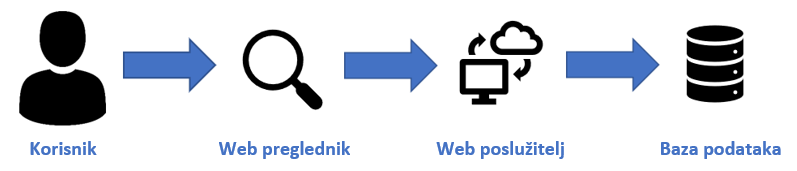
\includegraphics[width=1\linewidth]{"slike/arhitekturaApp.png"}
					\caption{Arhitektura sustava}
					\label{fig:arhitektura-sustava}
				\end{figure}

Prilikom pristupa web aplikaciji korisniku na jednostavan način postaje moguće pretražiti putovanja s odabranog polazišnog stajališta i kupiti kartu. Da bi korisnik mogao pristupiti navedenim funkcionalnostima treba pristupiti web pregledniku koji za njega vrši daljnju interakciju s ostalim podsustavima koji su sastavni dijelovi arhitekture sustava. Web preglednik dalje mora komunicirati s web poslužiteljem na kojem je sama implementacija web aplikacije. Preko web poslužitelja se obavljaju svi mogući funkcionalni zahtjevi aplikacije koji su prethodno definirani, a oni su izravno povezani s poslužiteljem baze podataka. U bazi podataka pohranjeni su svi podaci nužni za potpuno ispravan rad aplikacije, ali i podaci koje ručno unose korisnici poput osobnih podataka. Web poslužitelj šalje objekte na zahtjev klijenata, ti se zahtjevi realiziraju u obliku HTTP poruka. Web poslužitelju se pristupa preko nekog web preglednika.

Za izradu frontend dijela web aplikacije korišten je programski jezik Javascript s razvojnim okvirom React.js. Za izradu backend dijela korišten je Typescript s razvojnim okvirom Express.js. Baza podataka je implementirana pomoću PostrgreSQL.

 Za realizaciju arhitekture sustava korišten je koncept Model-View-Controller. Model–View–Controller je obrazac koji razdvaja aplikaciju u tri glavne
logičke komponente: Model, View i Controller. Svaka od nabrojenih komponenti ima zadatak rukovati s određenim razvojnim aspektima aplikacije. Također, one
su nezavisne jedna od druge i kao rezultat toga je jednostavno dodavanje i preoblikovanje svojstava.

\begin{figure}[H]
					\centering
					\includegraphics[width=0.7\linewidth]{"slike/MVC"}
					\caption{Model-View-Controller}
					\label{fig:Model-View-Controller}
				\end{figure}

• \textbf{Model}
Poznat je kao najniža razina što znači da je odgovoran za održavanje podataka s kojima korisnik radi. Glavni zadatak je dohvat, manipulacija podatcima odnosno suradnja s bazom podataka. 
Sprema tražene podatke u objekte i na taj način ih šalje bazi podataka. Reagira na zahtjeve Controllera jer on nikada sam ne razgovara s bazom podataka i nakon komunikacije
prosljeđuje potrebne podatke Controller-u. Jedna od bitnijih stvari za napomenuti je da Model nikada izravno ne komunicira s View.

• \textbf{View}
Služi za prikazivanje podataka tako što generira korisničko sučelje za korisnika. Ti podaci su rezultat rada Model-a, ali se oni ne preuzimaju izravno nego putem Controller-a tako da View surađuje samo s Controller-om.

•\textbf{Controller} 
Upravlja komponentama Model i View. Ne mora
brinuti o rukovanju logikom podataka, već samo govori Model-u što treba učiniti. Nakon primanja podataka od Model-a, on ih obrađuje i prosljeđuje rezultat do View-a.}

		
		\section{Baza podataka}
			
			
		{Za potrebe našeg sustava odabrali smo relacijsku bazu podataka koja nam olakšava modeliranje stvarnog svijeta. Baza je definirana skupom tablica, odnosno relacija koje su definirane svojim imenima i skupovima atributa (i ključevima). Zbog pouzdanosti, jednostavnosti i zadovoljavajućih preformansi, odabrali smo rad s PostreSQL bazom. Baza podataka omogućava nam brz i lak dohvat i spremanje podataka, odnosno obradu i izmjenu podataka korištenih u aplikaciji. Naša baza sastoji se od sljedećih entiteta: }
			\begin{packed_item}
				\item \text{User}
				\item \text{Ticket}
				\item \text{Journey}
				\item \text{TrainRoute}
				\item \text{Station}
				\item \text{SensorData}
			\end{packed_item}
		
			\subsection{Opis tablica}
			

\textbf{User}{ - Entitet User sadrži sve potrebne informacije o korisniku aplikacije koji može biti kupac ili administrator što određuje atribut UserType. User ima također i atribute firstName, lastName, email, password te createdDate što označava datum registracije korisnika. Email je jedinstven atribut, tako da se svaki User razlikuje po svom e-mailu. Ključ entiteta je email. }
				
				
				\begin{longtblr}[
					label=none,
					entry=none
					]{
						width = \textwidth,
						colspec={|X[6,l]|X[6, l]|X[20, l]|}, 
						rowhead = 1,
					} %definicija širine tablice, širine stupaca, poravnanje i broja redaka naslova tablice
					\hline \multicolumn{3}{|c|}{\textbf{Korisnik}}	 \\ \hline[3pt]
					\SetCell{LightGreen}email & VARCHAR	& jedinstveni e-mail korisnika   	\\ \hline
					firstName	& VARCHAR & ime korisnika \\ \hline 
					lastName & VARCHAR &  prezime korisnika \\ \hline 
					password & VARCHAR	&  lozinka registriranog korisnika	\\ \hline 
					role&VARCHAR&vrsta korisnika,može biti kupac ili administrator\\ \hline 
					createdDate&DATE&datum registracije korisnika 	\\ \hline 
				\end{longtblr}





\textbf{Ticket}{ - Entitet Ticket je slabi entitet koji ovisi o entitetu User iz razloga što karta ne može biti izdana bez da korisnik zatraži njezino izdavanje. Ključ entiteta Ticket je Id ticket-a. Atribut passengerEmail je strani ključ koji referencira entitet User te se radi o \textit{Many-to-Many} vezi. Atribut idJourney rute je strani ključ koji referencira entitet Journey te se radi o \textit{Many-To-One} vezi. }

				\begin{longtblr}[
					label=none,
					entry=none
					]{
						width = \textwidth,
						colspec={|X[6,l]|X[6, l]|X[20, l]|}, 
						rowhead = 1,
					} %definicija širine tablice, širine stupaca, poravnanje i broja redaka naslova tablice
					\hline \multicolumn{3}{|c|}{\textbf{Ticket}}	 \\ \hline[3pt]
					\SetCell{LightGreen}Id & INT	&  	jedinstveni identifikacijski broj karte koja je kupljena  	\\ \hline
					\SetCell{LightBlue} userId	& INT & strani ključ entiteta User 	\\ \hline 
					\SetCell{LightBlue} idJourney	& INT & strani ključ entiteta Journey \\ \hline
					passenger-Name	& VARCHAR & ime kupca karte \\ \hline 
					passenger-Surname & VARCHAR &  prezime kupca karte \\ \hline 
					wagon & INT	&  vagon za koji je kupljena karta \\ \hline
					wagonPosition & INT	&  pozicija vagona na kolodvoru	\\ \hline
					travelDate&DATE&datum putovanja 	\\ \hline
				\end{longtblr}
				
				


				\textbf{Journey} {- Ovaj entitet sadržava sve važne podatke za jedno putovanje vlakom. Sadrži atribute: IdJourney, departureTime i arrivalTime, price, departureStationName, arrivalStationName, routeId i sensorDataId. Atributi departureStationName i arrivalStationName su strani ključevi koji referenciraju entitet Station te se radi o \textit{Many-To-One} vezi. Atributi IdTrainRoute i sensorDataId su strani ključevi koji refenciraju entitet TrainRoute i SensorData putem \textit{Many-To-One} veze. }
				
				
				\begin{longtblr}[
					label=none,
					entry=none
					]{
						width = \textwidth,
						colspec={|X[6,l]|X[6, l]|X[20, l]|}, 
						rowhead = 1,
					} %definicija širine tablice, širine stupaca, poravnanje i broja redaka naslova tablice
					\hline \multicolumn{3}{|c|}{\textbf{Journey}}	 \\ \hline[3pt]
					\SetCell{LightGreen}idJourney & INT	&  	jedinstveni identifikacijski broj putovanja  	\\ \hline
					departureTime	& DATETIME &	datum i vrijeme polaska s polazišnog stajališta	\\ \hline 
					arrivalTime & DATETIME &	datum i vrijeme dolaska na odredišno stajalište	\\ \hline 
					price & FLOAT	&  	cijena karte za putovanje	\\ \hline 
					\SetCell{LightBlue} departure-StationName	&          VARCHAR &   	početno stajalište putovanja i strani ključ entiteta Station	\\ \hline 
					\SetCell{LightBlue} arrival-StationName	&        VARCHAR &   	završno stajalište putovanja	 i strani ključ entiteta Station	\\ \hline 
					\SetCell{LightBlue} idTrainRoute	& INT &   	jedinstveni identifikacijski broj TrainRoute-e	\\ \hline 
					sensorDataId	& INT &   	jedinstveni identifikacijski broj sensorData	\\ \hline
				\end{longtblr}
				
				





\textbf{TrainRoute} {- Entitet TrainRoute ima atribute: idTrainRoute, departureTime, arrivalTime, trainId i dates. U ruti Zagreb-Karlovac-Knin-Split, početak cjelokupne rute je Zagreb, a završetak Split. Entitet TrainRoute će imati sve moguće kombinacije podruta za primjer navedene rute. Journeys navedene rute će biti Zagreb-Karlovac, Zagreb-Knin, Zagreb-Split, Karlovac-Knin, Karlovac-Split, Knin-Split. Zbog potrebe zadatka da za svako putovanje imamo početno i završno odredište cjelokupne rute tog putovanja, nastao je ovaj entitet TrainRoute koji je povezan s Journeys \textit{One-To-Many} vezom. }
				
				
				\begin{longtblr}[
					label=none,
					entry=none
					]{
						width = \textwidth,
						colspec={|X[6,l]|X[6, l]|X[20, l]|}, 
						rowhead = 1,
					} %definicija širine tablice, širine stupaca, poravnanje i broja redaka naslova tablice
					\hline \multicolumn{3}{|c|}{\textbf{TrainRoute}}	 \\ \hline[3pt]
					\SetCell{LightGreen}IdTrainRoute & INT	&  	jedinstveni identifikacijski broj cjelokupne rute  	\\ \hline
					departureTime	& DATETIME &	datum i vrijeme polaska s polazišnog stajališta	\\ \hline 
					arrivalTime & DATETIME &	datum i vrijeme dolaska na odredišno stajalište	\\ \hline 
					trainId & INT	& jedinstveni identifikacijski broj vlaka koji vozi tu rutu 	\\ \hline 
					dates & DATETIME & datum vožnji vlaka \\ \hline
					
				\end{longtblr}

				\textbf{Station} {- Ovaj entitet sadržava imena svih stajališta. Entitet Stajalište povezan je putem dvije \textit{One-To-Many} veze s entitetom Putovanje, gdje jedna veza označava početno stajalište, a druga završno. }
				
				
				\begin{longtblr}[
					label=none,
					entry=none
					]{
						width = \textwidth,
						colspec={|X[6,l]|X[6, l]|X[20, l]|}, 
						rowhead = 1,
					} %definicija širine tablice, širine stupaca, poravnanje i broja redaka naslova tablice
					\hline \multicolumn{3}{|c|}{\textbf{Station}}	 \\ \hline[3pt]
					\SetCell{LightGreen}name & VARCHAR	&  	ime stajališta 	\\ \hline
				\end{longtblr}

				\textbf{SensorData} {- Ovaj entitet sadržava sve važne podatke za jedno mjerenje senzora. Sadrži atribute: id, time, speed, measurments, stationName, idJourney, idTrainRoute i travelDate. Entitet SensorData povezan je putem \textit{Many-To-One} veze s entitetom Journey. }
				
				
				\begin{longtblr}[
					label=none,
					entry=none
					]{
						width = \textwidth,
						colspec={|X[6,l]|X[6, l]|X[20, l]|}, 
						rowhead = 1,
					} %definicija širine tablice, širine stupaca, poravnanje i broja redaka naslova tablice
					\hline \multicolumn{3}{|c|}{\textbf{SensorData}}	 \\ \hline[3pt]
					\SetCell{LightGreen}id & INT	&  	jedinstveni identifikacijski broj mjerenja  	\\ \hline
					time & DATETIME & datum i vrijeme mjerenja senzora	\\ \hline 
					measurments & VARCHAR &	vrijednost mjerenja senzora	\\ \hline 			
					speed & INT &  	brzina vlaka u trenutku mjerenja senzora	\\ \hline 
					stationName	& VARCHAR &   	stanica koju je vlak prošao uz senzor	\\ \hline
					travelDate & DATE & datum putovanja vlaka koji prolazi kraj senzora  \\ \hline 
					\SetCell{LightBlue} idJourney	& INT &   	strani ključ entiteta Journey	\\ \hline 
					\SetCell{LightBlue} idTrainRoute	& INT &   	strani ključ entiteta TrainRoute	\\ \hline 
				\end{longtblr}
				
				

			\subsection{Dijagram baze podataka}

	
				% TODO: \usepackage{graphicx} required
				\begin{figure}[H]
					\centering
					\includegraphics[width=1\linewidth]{"slike/dijagramBaze"}
					\caption{Dijagram baze podataka}
					\label{fig:dijagram-bp}
				\end{figure}
			
			\eject
			
			
		\section{Dijagram razreda}
		
	

				% TODO: \usepackage{graphicx} required
				\begin{figure}[H]
					\centering
					\includegraphics[width=1\linewidth]{"slike/ModelClassDiagram"}
					\caption{Dijagram razreda Modela}
					\label{fig:dijagram-model}
				\end{figure}

				{Model razredi preslikavaju strukturu baze podataka u aplikaciji. Implementirane metode direktno komuniciraju s bazom podataka te vraćaju tražene podatke. Razred \textit{User} predstavlja registriranog i prijavljenog korisnika koji može koristiti njegove osnovne funkcionalnosti. Razred \textit{Ticket} predstavlja jednu kartu koju je kupio \textit{User} za jedno putovanje - \textit{Journey}. Razred \textit{Journey} predstavlja relaciju putovanja za koju korisnik(\textit{User}) kupuje željezničku kartu. Razred \textit{TrainRoute} predstavlja kompletnu rutu na kojoj putuje vlak na kojem je korisnik kupio kartu za određeno putovanje. Razred \textit{Station} predstavlja listu svih stajališta kojima vozi naš prijevoznik, a razred \textit{SensorData} predstavlja mjerenja sustava senzora Gotcha za svako putovanje.}

				% TODO: \usepackage{graphicx} required
				\begin{figure}[H]
					\centering
					\includegraphics[width=1\linewidth]{"slike/ControllerClassDiagram"}
					\caption{Dijagram razreda Controllera}
					\label{fig:dijagram-controller}
				\end{figure}
				{Dijagram se sastoji od 8 nadglednika: HomeController, LoginController, RegisterController, AdminController, PaymentController, SensorController, SettingsController, TimetableController te svi naslijeđuju apstraktni razred Controller. U serveru se inicijaliziraju svi kontroleri (stavljaju u listu). HomeController se koristi prilikom ulaska korisnika na Home ekran i prikaz voznog reda na stranici. RegisterController se koristi prilikom registracije korisnika na stranicu, a LoginController prilikom prijave korisnika/admina u stranicu. AdminController se koristi prilikom funkcionalnosti koje su omogućene za Admina(pregleda, brisanje korisnika).	SensorController se koristi prilikom dohvata i obrade podataka sa senzora. PaymentController služi za obradu plaćanja prilikom kupnje karta te sprema podatke o transakcijama. SettingsController koristimo pri dohvatu podataka korisnika te brisanju njegova računa. TimetableController koristimo pri dohvatu putovanja za odabranu odlaznu i dolaznu stanicu i datum.	}
			
			\eject

\section{Dijagram stanja}
			{Dijagram stanja opisuje dinamičko ponašanje dijela sustava u vremenu. Ono sadrži konačan broj stanja i prijelaza među stanjima temeljenima na događajima. Na slici je prikazan dijagram stanja za sve uloge korisnika: konkretnog korisnika i administratora. Početno stanje neregistriranog korisnika (odnosno neprijavljenog) vodi u stanje prijave. Neregistriranim korisnicima je ostavljena mogućnost registracije, nakon čega je prijavom moguće doći do početne stranice aplikacije. Uloga korisnika razdjeljuje stanje početne stranice na dva unutarnja. Administratorima je omogućena akcija prikaza svih korisnika, njihovog brisanja i ispisa njihovih transakcija. Konkretnim korisnicima je omogućena akcija ispisa nadolazećih vlakova na odabranu stanicu. Svi korisnici imaju i opciju prikaza voznog reda. Međutim, samo konkretni korisnici imaju opciju kupnje karte za odabrano putovanje. Da bi se izvršila kupnja potrebno je ispuniti obrazac (ukoliko nije upamćen jer se radi o prvoj transakciji) te ju potvrditi. Potvrdom se šalju dva e-maila, prvi za potvrdu o kupnji te drugi sa sadržajem karte i informacijama o odabranom putovanju. Iz svih stanja je moguće odjaviti se ili se vratiti u stanje početne stranice. } 
			
			 % TODO: \usepackage{graphicx} required
				\begin{figure}[H]
					\centering
					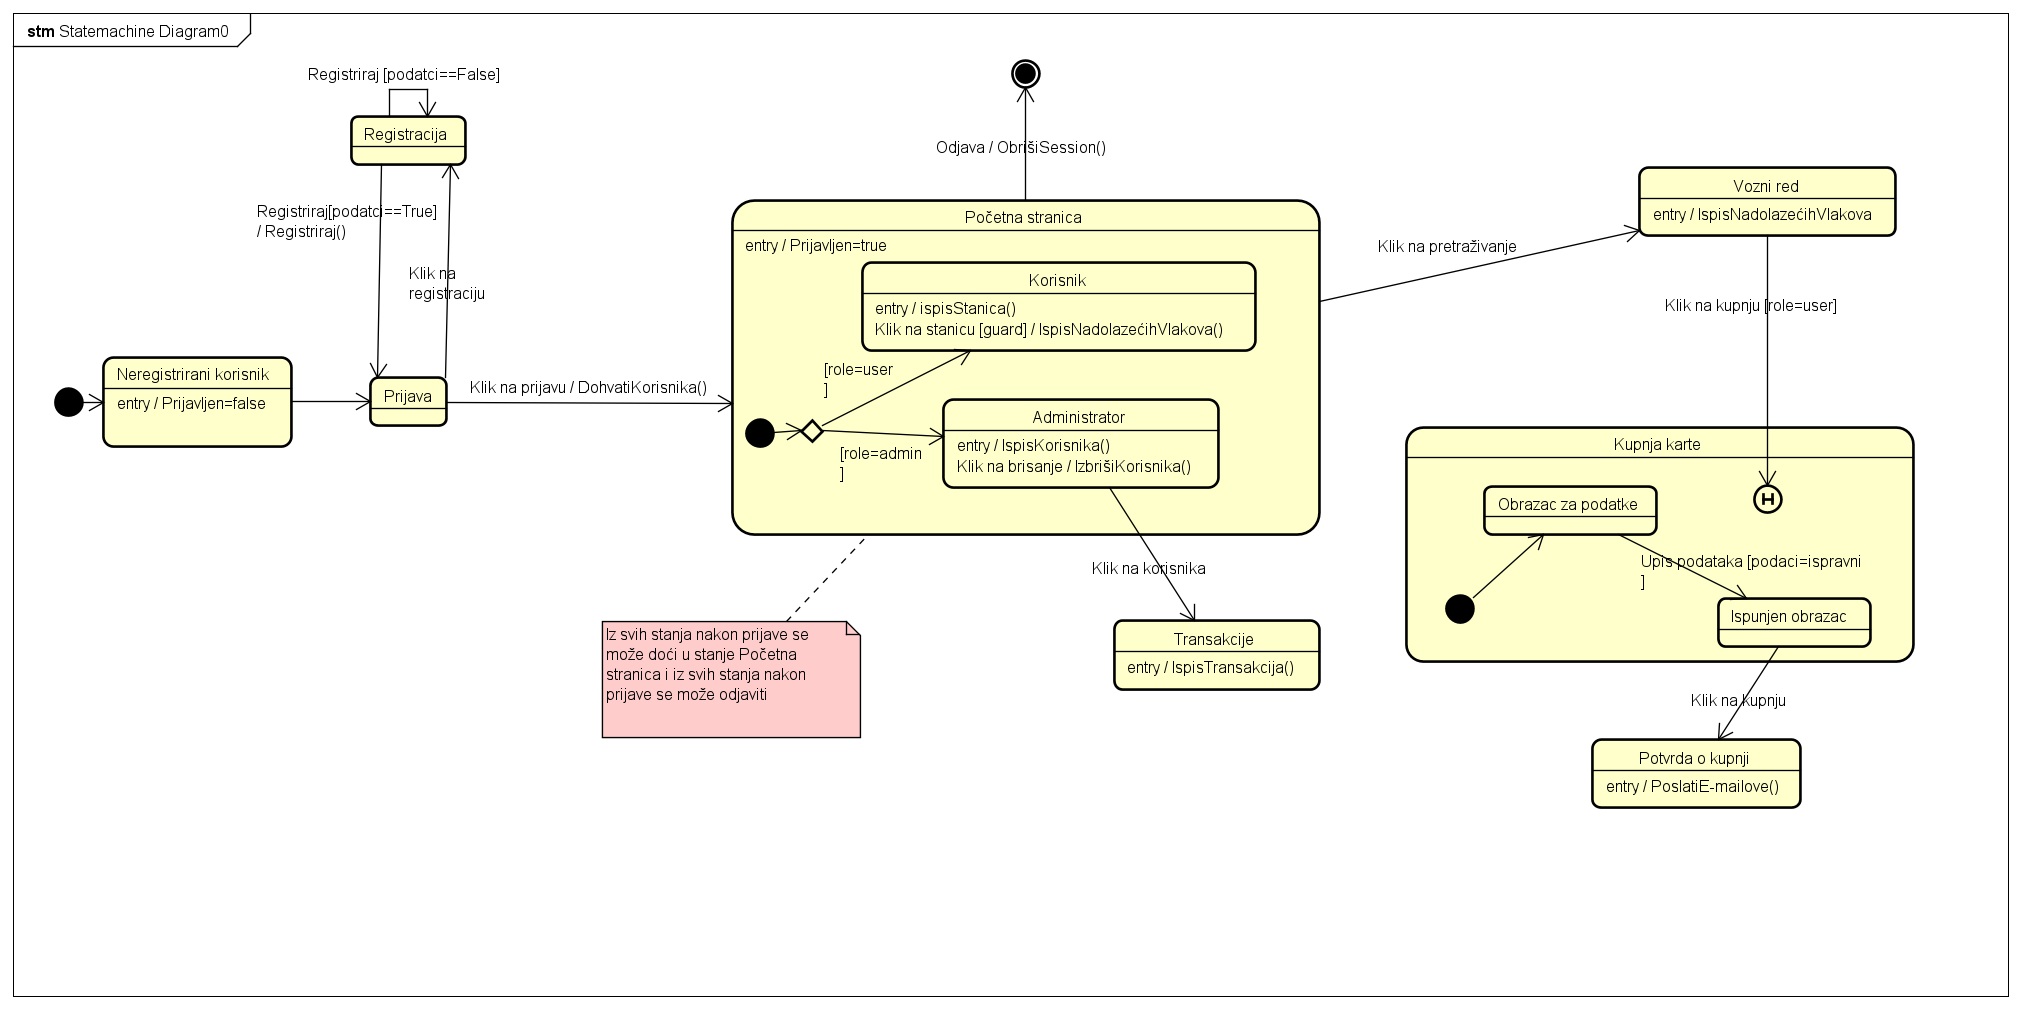
\includegraphics[width=1\linewidth]{"slike/StateMachineDiagram.png"}
					\caption{Dijagram stanja aplikacije}
					\label{fig:dij-state}
				\end{figure}
			
			
			\eject 
		
\section{Dijagram aktivnosti}

			{Dijagrami aktivnosti služe za modeliranje ponašanja nizom akcija, odnosno modeliranje toka i podataka. Pomaže nam pri zamišljanju redoslijeda aktivnosti i tijeka rada aplikacije. Na slici 4.7 prikazan je dijagram aktivnosti koji prikazuje procese pregledavanje i pretraživanje vlakova i voznih linija, odnosno kupnju karata za te linije. Korisnik se prijavljuje u sustav, zatim može pregledati vozni red pomoću odabira stanica i datuma polaska, te može pregledati koji vlakovi dolaze na označeno stajalište. Nakon odabira stanica i datuma dolazi do izlistanog voznog reda za te podatke pa odabire opciju kupnje. Zatim ispunjava obrazac za kartično plaćanje te potvrđuje svoju kupnju. Na slici 4.8 prikazan je dijagram aktivnosti administratora za brisanje korisnika i pregled njihovih transakcija. Nakon prijave, administrator dobiva izlistane korisnike za koje može odabrati brisanje ili pregled transakcija. Ukoliko odabere mogućnost brisanja, sustav će ga upozoriti i pitati je li siguran u brisanje toga klijenta. Administrator može prihvatiti brisanje ili odustati. Ako odabere pregled transakcija, aplikacija ga odvede na novu stranicu gdje su izlistane sve kupnje tog korisnika. }
			
			 % TODO: \usepackage{graphicx} required
				\begin{figure}[H]
					\centering
					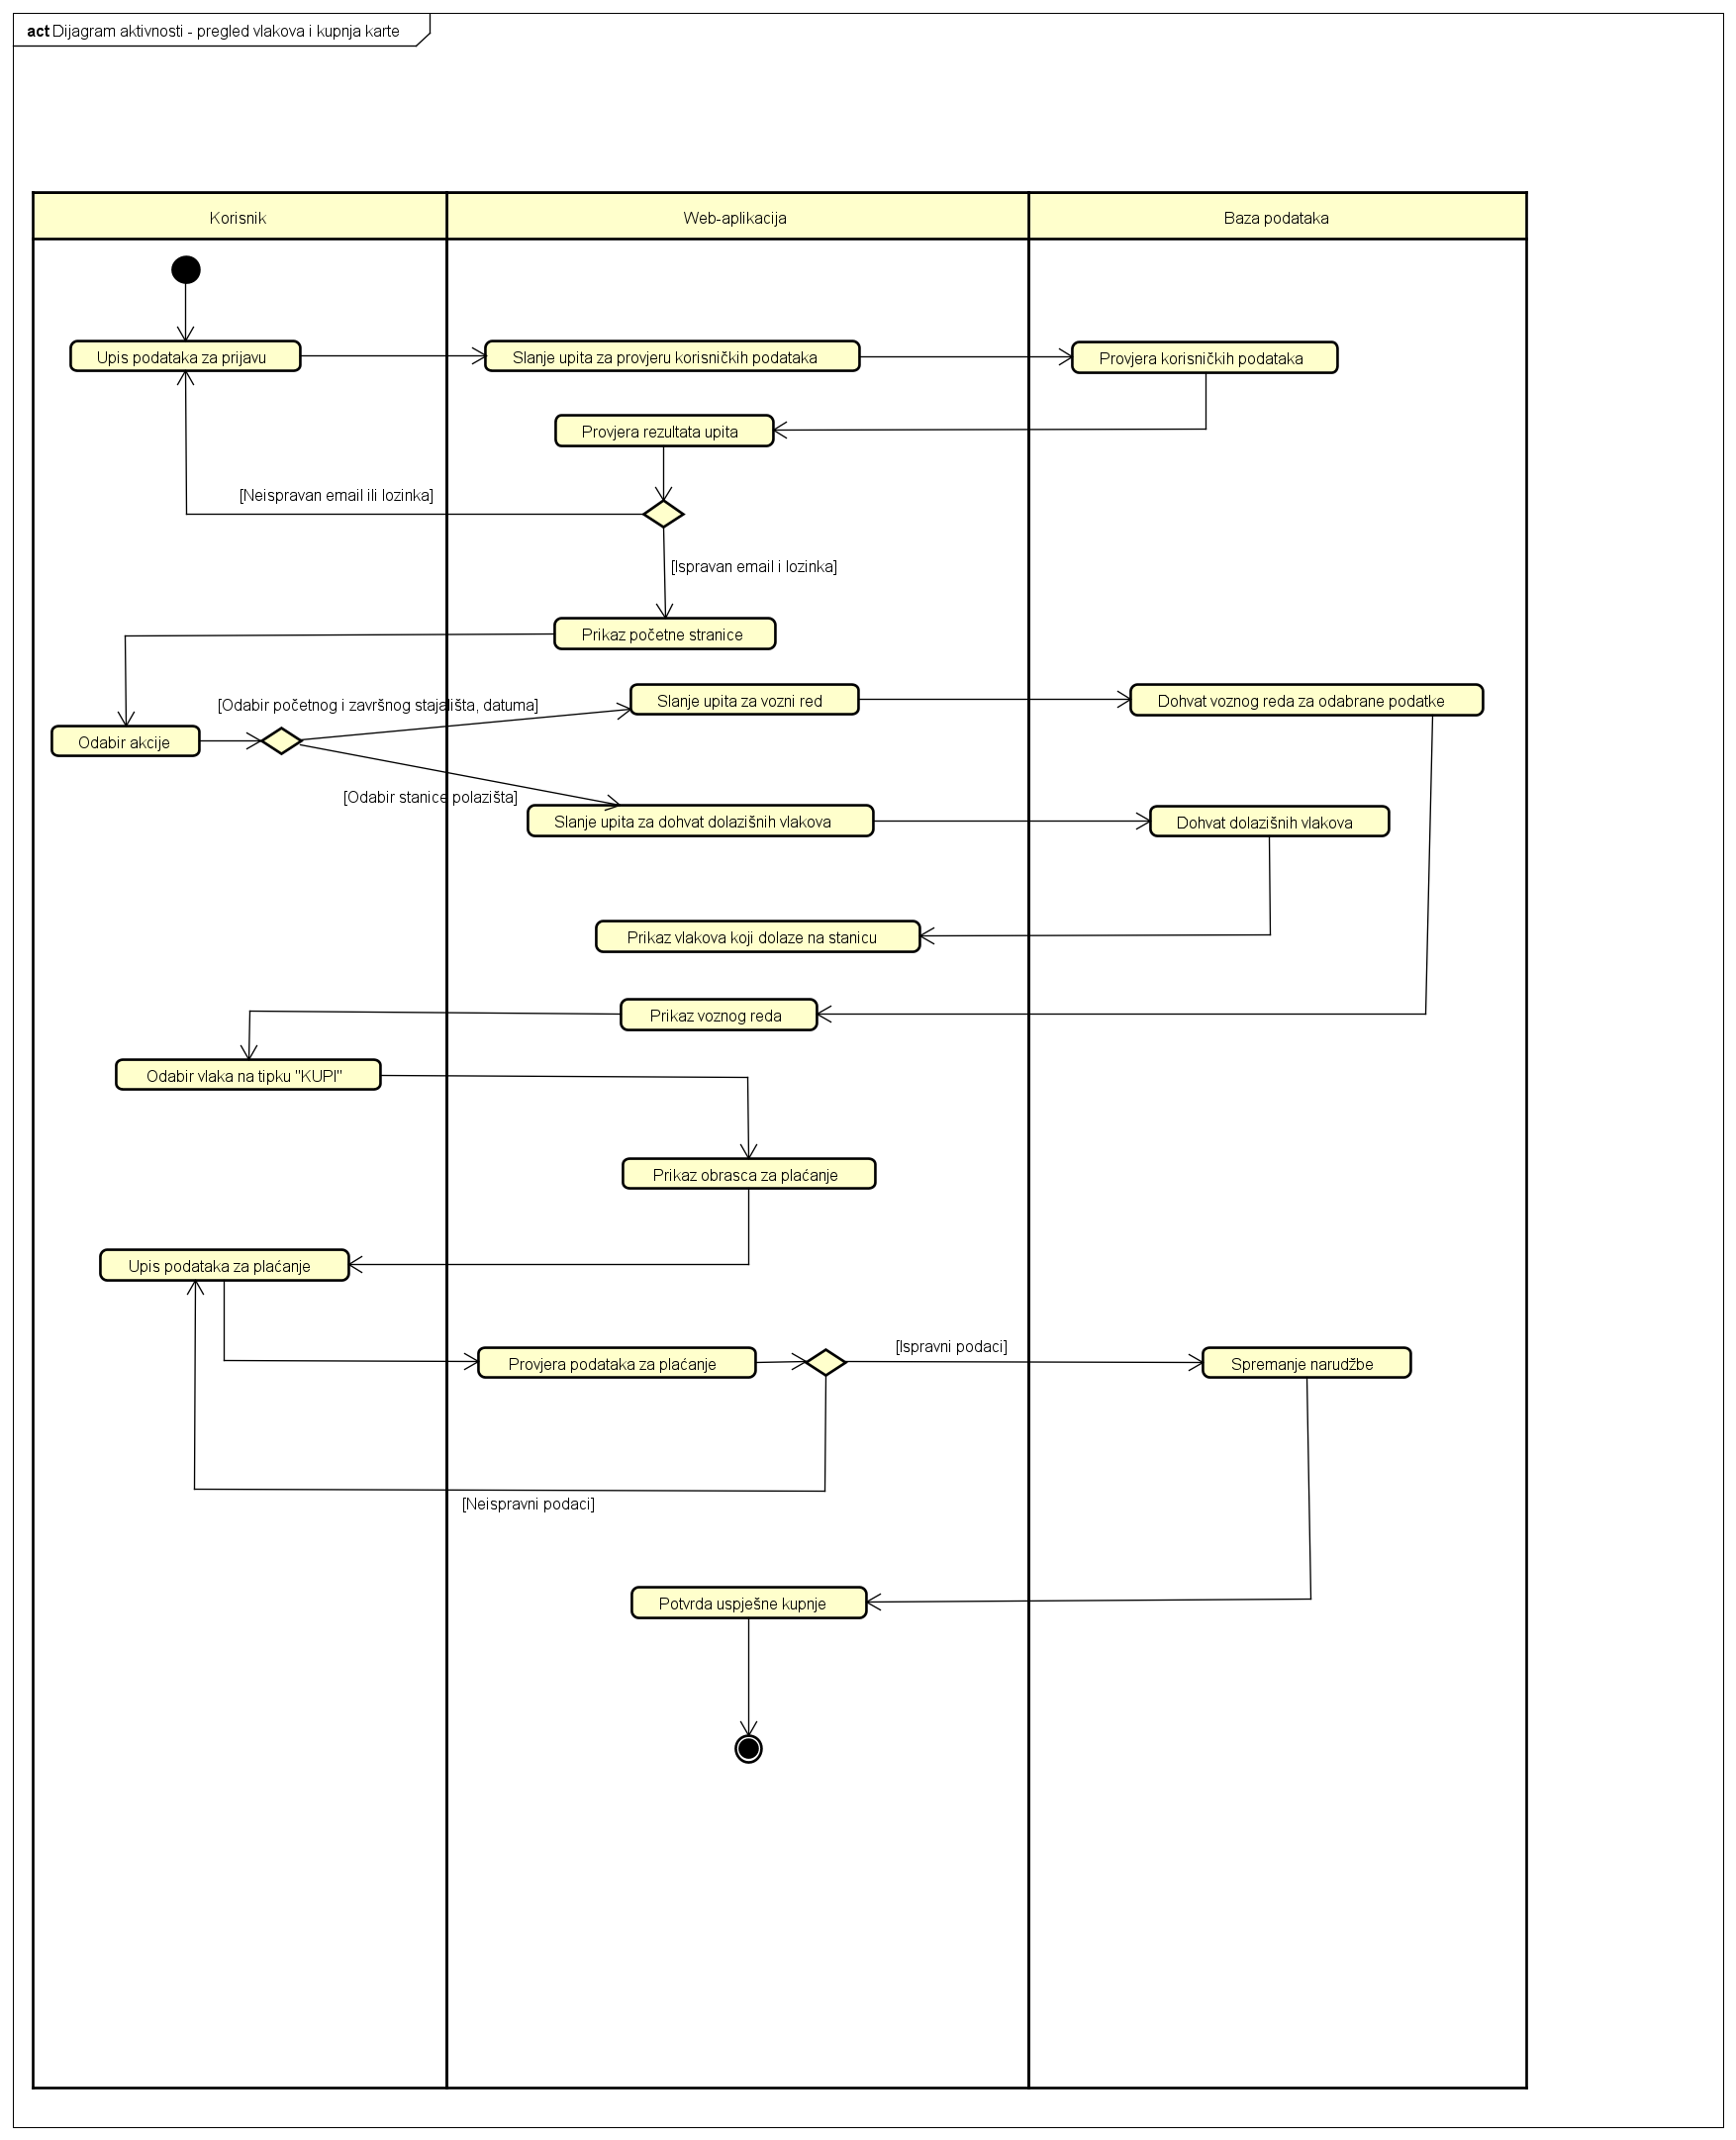
\includegraphics[width=1\linewidth]{"slike/actDiagram1.png"}
					\caption{Dijagram aktivnosti - Pregled vlakova i kupnja karte}
					\label{fig:dij-akt-prvi}
				\end{figure}
			
			% TODO: \usepackage{graphicx} required
				\begin{figure}[H]
					\centering
					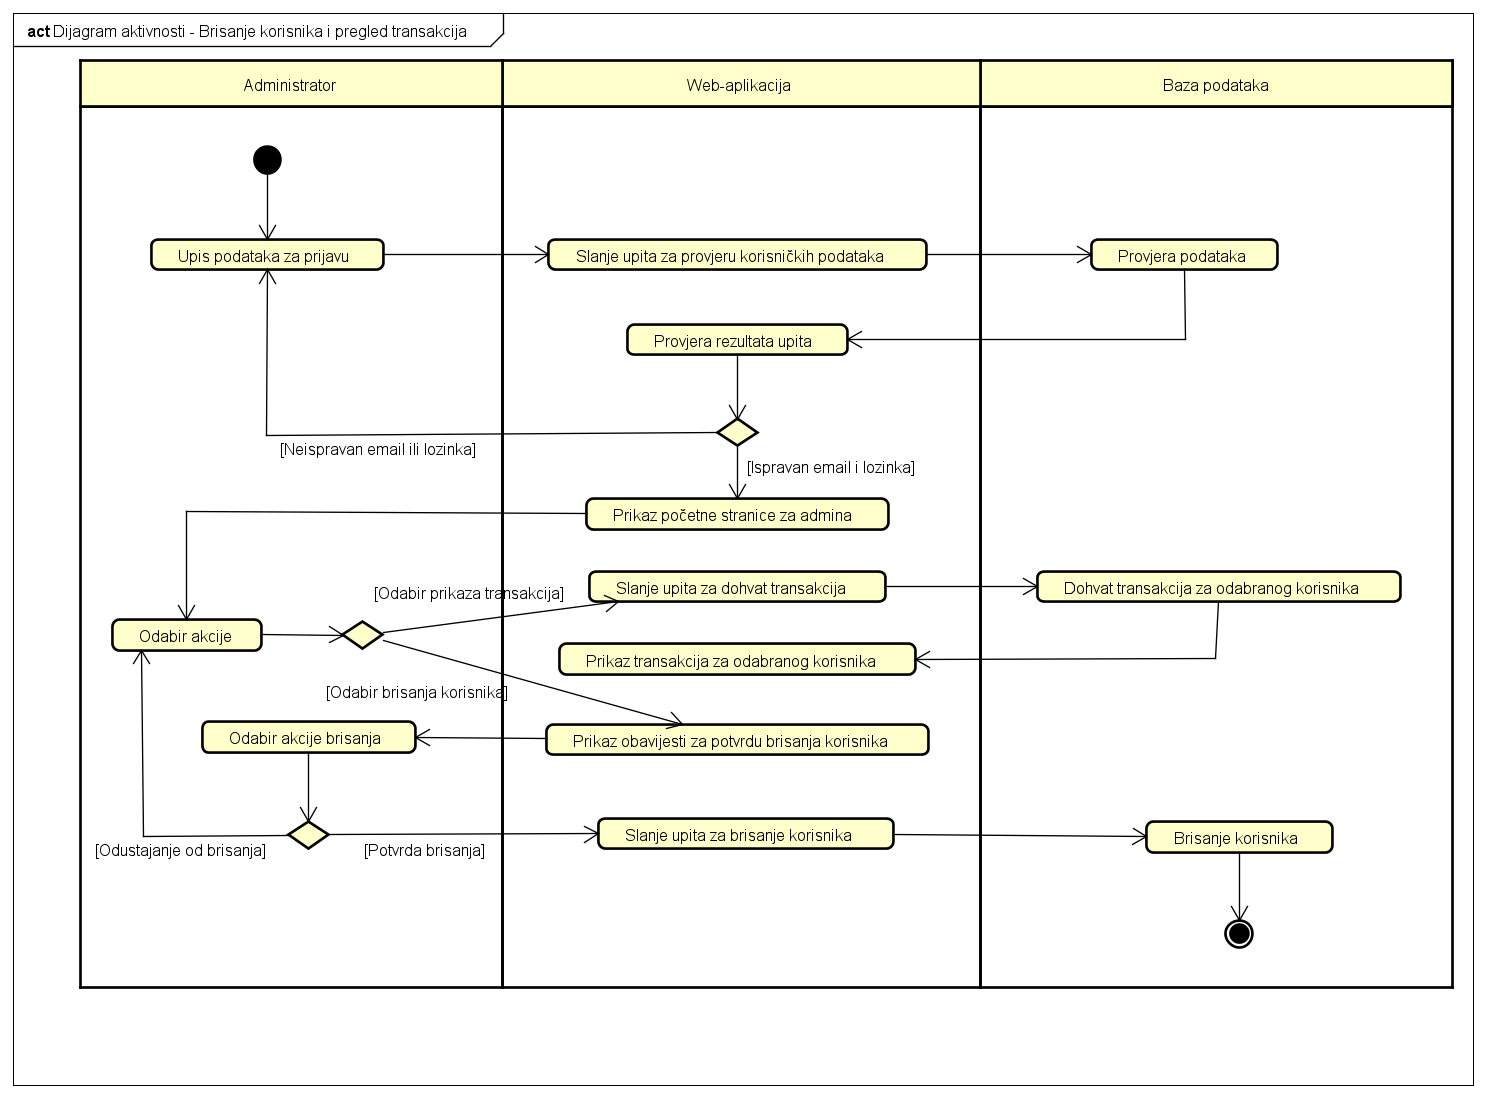
\includegraphics[width=1\linewidth]{"slike/actDiagram2.png"}
					\caption{Dijagram aktivnosti - Brisanje korisnika i pregled transakcija}
					\label{fig:dij-akt-drugi}
				\end{figure}
			
			\eject

\section{Dijagram komponenti}
			{Dijagramom komponenti se vizualizira organizacija i međuovisnost između implementacijskih komponenata te odnos programske potpore prema okolini. Pogodan je za uslužno-orijentiranu arhitekturu i sačinjen je od komponenti, sučelja i poveznica. Sučeljem za dohvat HTML, CSS i JS datoteka dohvaćaju se datoteke sa frontenda aplikacije. Komponentom Router poslužuju se komponente stranice i React biblioteke na upit s URL-a. Dohvatom JSON podataka pristupa se CRUDE REST API komponenti koja komunicira sa backendom aplikacije. Node-Postgres je kolekcija funkcija za komunikaciju Node.js-a i PostgresSQL-a. Pristigli podaci iz baze se šalju MVC arhitekturi u obliku Data transfer object-a.} 
			
			 % TODO: \usepackage{graphicx} required
				\begin{figure}[H]
					\centering
					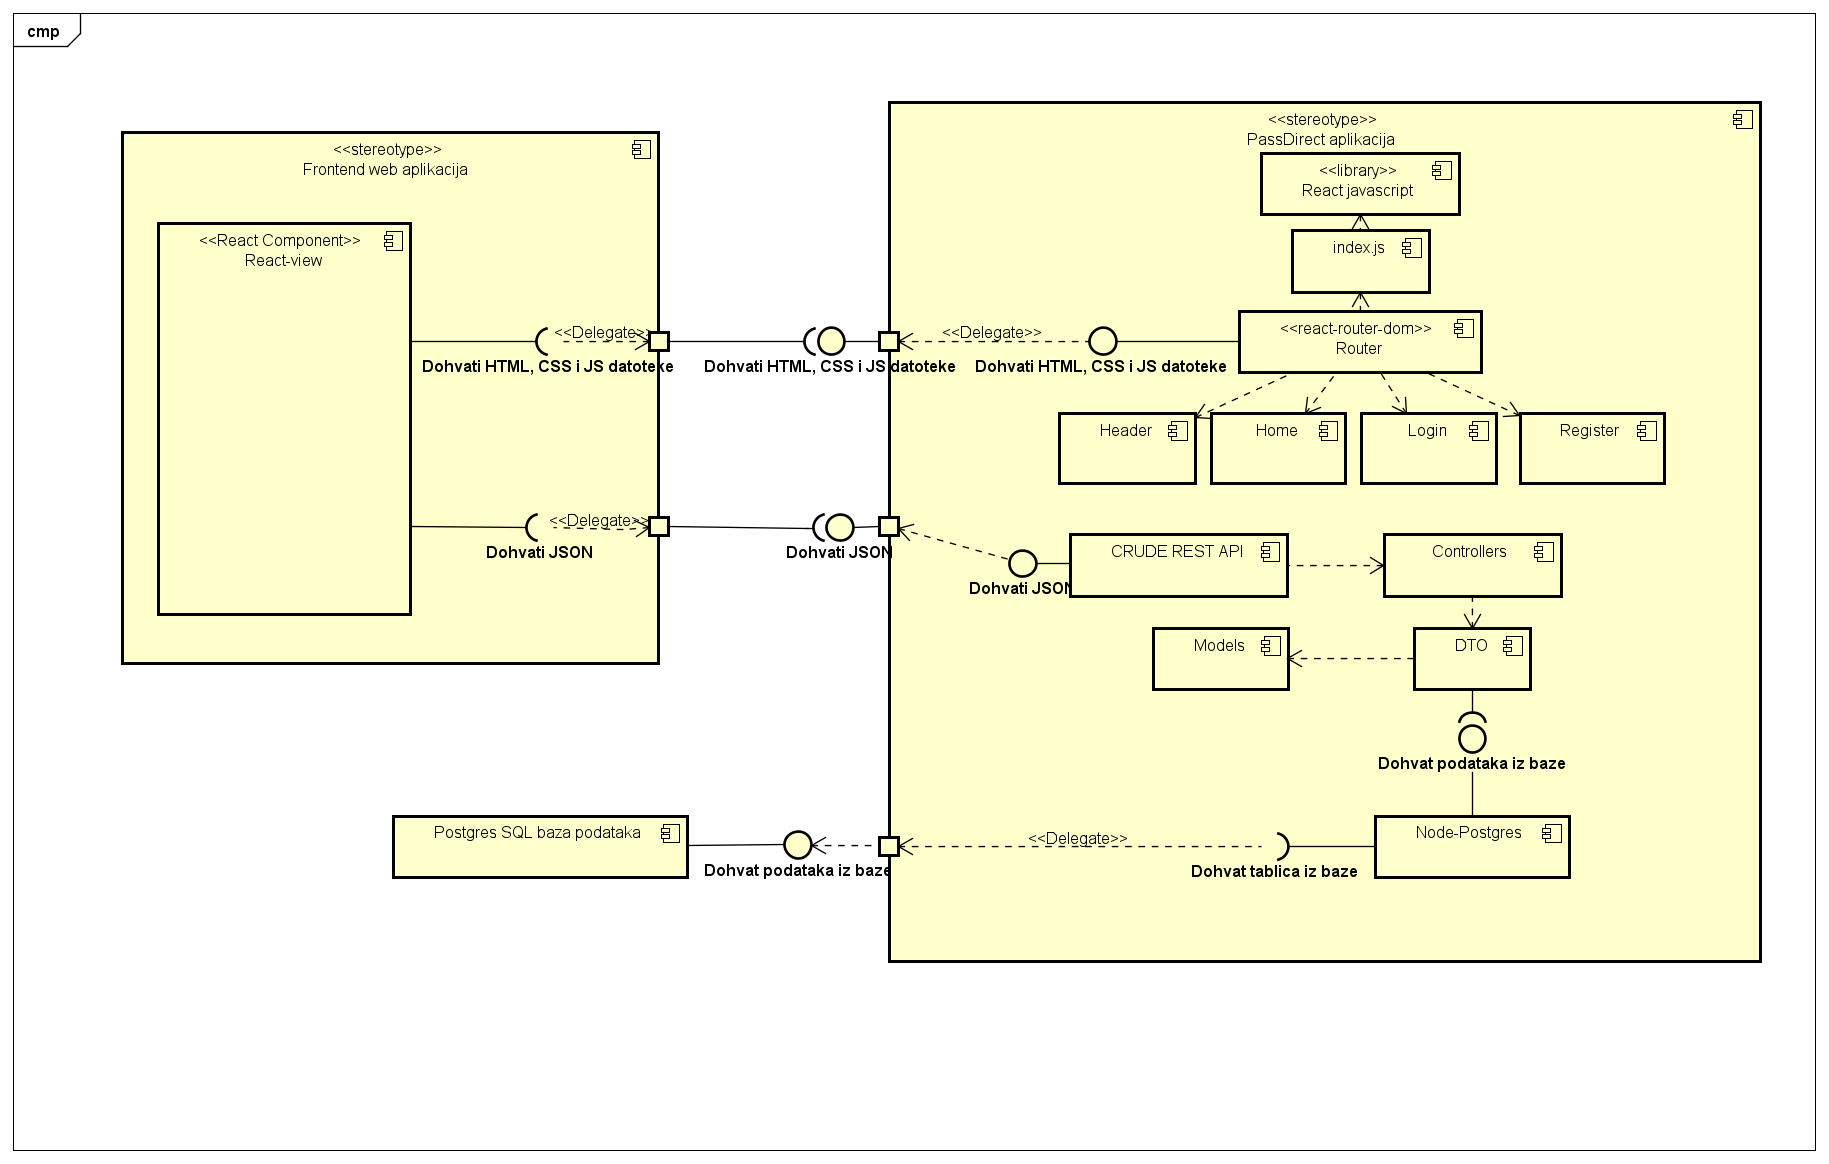
\includegraphics[width=1\linewidth]{"slike/ComponentDiagram.png"}
					\caption{Dijagram komponenti}
					\label{fig:dij-komponenti}
				\end{figure}
			
			
			\eject 
		
	\chapter{Implementacija i korisničko sučelje}
		
		
		\section{Korištene tehnologije i alati}
		
			{\hspace{7mm}\textbf{JavaScript} (https://www.javascript.com/)}\\
			
	{JavaScript je namijenjen omogućavanju dinamičnog načina stvaranja HTML elemenata i stvaranju interaktivnog sadržaja u HTML-u. Zajedno s CSS-om, JavaScript je osnova dinamičke web stranice.}\\

			{\textbf{TypeScript} (https://www.typescriptlang.org/)}\\
			
	{TypeScript je objektno orijentirani jezik, nadskup JavaScript-a koji se pri izvođenju prevodi u JavaScript, a u aplikaciji je korišten pri izradi \textit{backenda}.}\\

			{\textbf{CSS} (https://www.w3schools.com/css/)}\\
	
	{CSS koristimo za oblikovanje stila i izgleda stranice na način prilagođen zaslonu korisnika.}\\

			{\textbf{HTML} (https://html.com/)}\\
	
	{HTML je označni jezik pomoću kojega definiramo strukturu, sadržaj i funkcije web-stranica.}\\
	
			{\textbf{React} (https://reactjs.org/)}\\

	{React je JavaScript knjižnica koja nam nudi mogućnost opisivanja korisničkog sučelja komponentama koje je lako oblikovati i upravljati njima. Korišten je za izradu \textit{frontend} dijela aplikacije.\\

			{\textbf{PostreSQL} (https://www.postgresql.org/)}\\

	{PostreSQL je sustav za upravljanje bazom podataka otvorenog koda. Sprema podatke u zasebne tablice uz mogućnost naknadne obrade i pristupa podacima.}\\
			
			{\textbf{SQL} (https://www.w3schools.com/sql/)}\\

	{SQL je alat za organiziranje, upravljanje i preuzimanje podataka pohranjenih u bazi podataka korištenoj u PostreSQL-u.}\\

			{\textbf{Git} (https://git-scm.com/)}\\

	{Git je softver otvorenog koda korišten za kontroliranje verzija i praćenje promjena koda u aplikaciji koju izrađuje više korisnika.}\\

			{\textbf{GitLab} (https://about.gitlab.com/)}\\
	
	{GitLab je web platforma na kojoj se nalazi udaljeni repozitorij projekta i koja omogućuje lak uvid u promjene koda i dokumentacije, grafove aktivnosti i jednostavnu suradnju više sudionika projekta.}\\

			{\textbf{LaTeX} (https://www.latex-project.org/)}\\
	
	{LaTeX je softver koji omogućuje strukturirano slaganje i pripremu tekstova s opcijom formatiranja u oblik pogodan za pregled ili ispis.}\\

			{\textbf{Astah} (https://astah.net/)}\\

	{Astah je alat koji se koristio za izradu UML dijagrama.}\\
	
			{\textbf{Heroku} (https://www.heroku.com/)}\\
	
	{Heroku je web platforma koja omogućuje postavljanje i upravljanje web-aplikacijama.}\\
	
			{\textbf{WhatsApp} (https://www.whatsapp.com/)}\\

	{WhatsApp je aplikacija koja je korištena svakodnevno za lakšu komunikaciju i razmjenu ideja, problema.}\\

			{\textbf{Microsoft Teams} (https://www.microsoft.com/hr-hr/microsoft-teams/group-chat-software)}\\

	{Teams je aplikacija koja je korištena za e-sastanke i jedan dio pomoćne dokumentacije.}\\

	{\textbf{Postman} (https://www.postman.com/)}\\
			
	{Postman je API platforma namijenjena za korištenje API-ja. Njime se pojednostavljuju API lifecycle-i radi brže i jednostavnije izgradnje.}\\

	{\textbf{PostHook} (https://posthook.io/)}\\

	{Servis PostHook koristimo kako bismo ostvarili slanje POST zahtjeva s vremenskom odgodom. Pomoću ovog servisa simuliramo slanje sa senzora tijekom vožnje vlaka. Koristeći servis Postman, na PostHook šaljemo podatke koje smo definirali kao iščitanja senzora, uz dodatne metapodatke s informacijom o zakazanom vremenu slanja danog podatka, ruti za slanje, itd. Servis Posthook dalje čeka definirano vrijeme slanja te prosljeđuje unesene podatke na rutu koju smo zadali. }


			\eject 
		
	
		\section{Ispitivanje programskog rješenja}
			
			\subsection{Ispitivanje komponenti}
		
			
			\noindent \textbf {Ispitni slučaj 1: Testiranje funkcije validateEmail}\\
			\noindent \textbf {Ulaz:} "IspravanEmail123@email.com".\\
			\noindent \textbf {Očekivani rezultat:} Funkcija vraća \textit{true} jer je format e-maila dozvoljen.\\
			\noindent \textbf {Rezultat:} Očekivani rezultat je zadovoljen. \textcolor{green}{Metoda je prošla test.}\\
			
			% TODO: \usepackage{graphicx} required
				\begin{figure}[H]
					\centering
					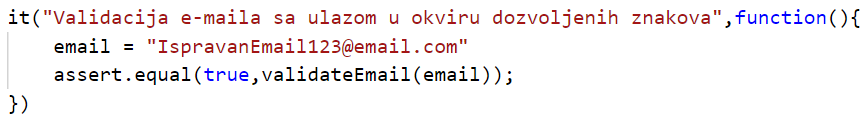
\includegraphics[width=1\linewidth]{"slike/ispravnaValidacija.png"}
					\caption{Ispravna validacija}
					\label{fig:da-val}
				\end{figure}
			

			

			\noindent \textbf {Ispitni slučaj 2: Testiranje funkcije validateEmail}\\
			\noindent \textbf {Ulaz 1:} "NeispravanEmail.com".\\
			\noindent \textbf {Ulaz 2:} "NeispravanEmail@domena".\\
			\noindent \textbf {Ulaz 3:} "NeispravanEmail@domena.a".\\
			\noindent \textbf {Ulaz 4:} "NeispravanEmail@domena.123".\\
			\noindent \textbf {Očekivani rezultati:} Funkcija vraća \textit{false} za svaki od ulaza jer su formati e-maila nedozvoljeni.\\
			\noindent \textbf {Rezultat:} Očekivani rezultat je zadovoljen. \textcolor{green}{Metoda je prošla test.}\\
			
			% TODO: \usepackage{graphicx} required
				\begin{figure}[H]
					\centering
					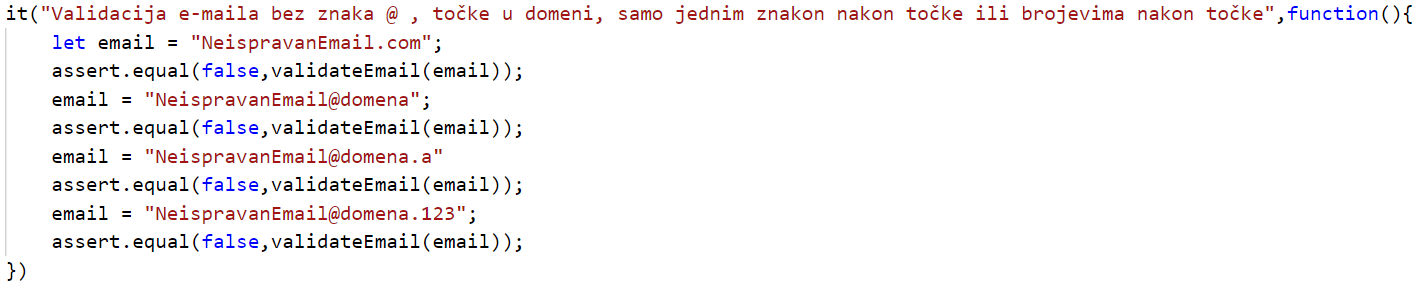
\includegraphics[width=1\linewidth]{"slike/neispravnaValidacija.png"}
					\caption{Validacija neispravno formatiranog e-maila}
					\label{fig:ne-val}
				\end{figure}
			
			\eject


			\noindent \textbf {Ispitni slučaj 3: Testiranje funkcije validateEmail}\\
			\noindent \textbf {Ulazi:} znak+"@email.com", znak = "<", ">", "(", ")", "[", "]", ".", ",", ";", ":", " ", "@", """.\\
			\noindent \textbf {Očekivani rezultat:} Funkcija vraća \textit{false} za svaki od ulaza jer je format e-mailova nedozvoljen.\\
			\noindent \textbf {Rezultat:} Očekivani rezultat je zadovoljen. \textcolor{green}{Metoda je prošla test.}\\

			% TODO: \usepackage{graphicx} required
				\begin{figure}[H]
					\centering
					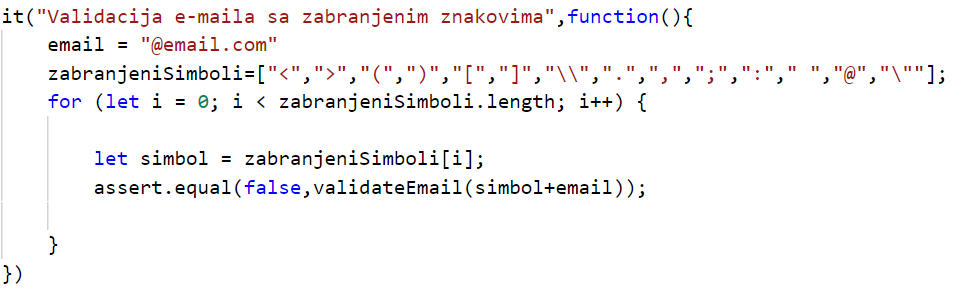
\includegraphics[width=1\linewidth]{"slike/validacijaSaZabranjenimZnakovima.png"}
					\caption{Validacija e-maila koji sadrži zabranjene znakove}
					\label{fig:zab-val}
				\end{figure}

			
			\noindent \textbf {Ispitni slučaj 4: Kalkulacija pozicije s ispravnim podacima}\\
			\noindent \textbf {Ulazi:} Podaci={"1":[10,9],"2":[12,23],"3":[6,0],"4":[2,9]}.\\
			\noindent \textbf {Očekivani rezultat:} Funkcija vraća vagon i poziciju u vagonu s najmanjim brojem ljudi ukoliko razlika putnika u ostalim vagonima nije 30 ili više.\\
			\noindent \textbf {Rezultat:} Očekivani rezultat je zadovoljen. \textcolor{green}{Metoda je prošla test.}\\

			% TODO: \usepackage{graphicx} required
				\begin{figure}[H]
					\centering
					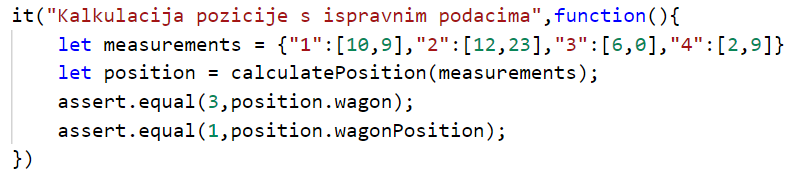
\includegraphics[width=1\linewidth]{"slike/kalkulacija1.png"}
					\caption{Kalkulacija s ispravnim podacima}
					\label{fig:isp-kal}
				\end{figure}

			\noindent \textbf {Ispitni slučaj 5: Kalkulacija pozicije s vlakom bez putnika }\\
			\noindent \textbf {Ulazi:} Podaci={"1":[0,0],"2":[0,0],"3":[0,0],"4":[0,0]}.\\
			\noindent \textbf {Očekivani rezultat:} Funkcija vraća stražnji dio prvog vagona.\\
			\noindent \textbf {Rezultat:} Očekivani rezultat je zadovoljen. \textcolor{green}{Metoda je prošla test.}\\

			% TODO: \usepackage{graphicx} required
				\begin{figure}[H]
					\centering
					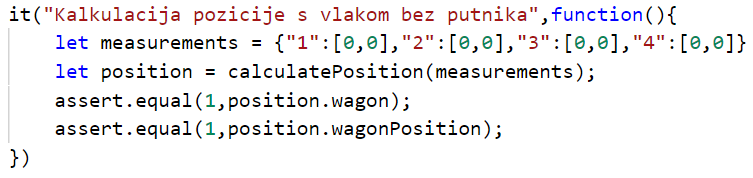
\includegraphics[width=1\linewidth]{"slike/kalkulacijaBezPutnika.png"}
					\caption{Kalkulacija bez putnika}
					\label{fig:nul-kal}
				\end{figure}
		
			\noindent \textbf {Ispitni slučaj 6: Kalkulacija pozicije s razlikom putnika većom od 30 u jednom vagonu }\\
			\noindent \textbf {Ulazi:} Podaci={"1":[0,30],"2":[20,24],"3":[15,20],"4":[18,26]}.\\
			\noindent \textbf {Očekivani rezultat:} Funkcija vraća vagon s razlikom od 30 putnika ili više.\\
			\noindent \textbf {Rezultat:} Očekivani rezultat je zadovoljen. \textcolor{green}{Metoda je prošla test.}\\

			% TODO: \usepackage{graphicx} required
				\begin{figure}[H]
					\centering
					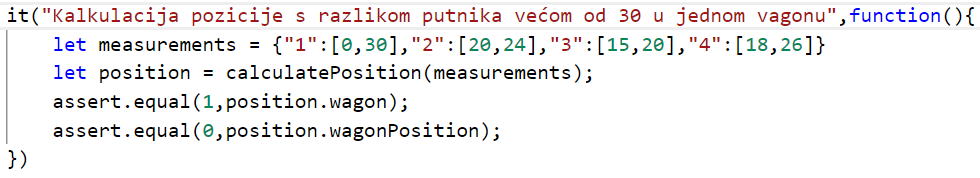
\includegraphics[width=1\linewidth]{"slike/kalkulacijaSRazlikomOd30.png"}
					\caption{Kalkulacija s razlikom od 30 putnika u jednom vagonu}
					\label{fig:j-kal}
				\end{figure}

			\noindent \textbf {Ispitni slučaj 7: Kalkulacija pozicije s razlikom putnika većom od 30 u više vagona }\\
			\noindent \textbf {Ulazi:} Podaci={"1":[0,30],"2":[60,94],"3":[31,58],"4":[50,73]}.\\
			\noindent \textbf {Očekivani rezultat:} Funkcija vraća vagon s najvećom razlikom.\\
			\noindent \textbf {Rezultat:} Očekivani rezultat je zadovoljen. \textcolor{green}{Metoda je prošla test.}\\

			% TODO: \usepackage{graphicx} required
				\begin{figure}[H]
					\centering
					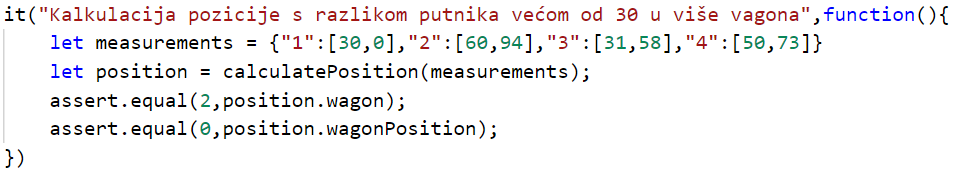
\includegraphics[width=1\linewidth]{"slike/kalkulacijaSRazlikomOd30uVise.png"}
					\caption{Kalkulacija s razlikom od 30 putnika u više vagona}
					\label{fig:v-kal}
				\end{figure}
			
			\noindent \textbf {Ispitni slučaj 8: Kalkulacija pozicije s neispravnim podacima}\\
			\noindent \textbf {Ulazi:} Podaci={"1":"Krivi podatak","2":"Krivi podatak","3":"Krivi podatak","4":"Krivi podatak"}.\\
			\noindent \textbf {Očekivani rezultat:} Funkcija izbacuje error o krivom podatku.\\
			\noindent \textbf {Rezultat:} Očekivani rezultat je zadovoljen. \textcolor{green}{Metoda je prošla test.}\\

			% TODO: \usepackage{graphicx} required
				\begin{figure}[H]
					\centering
					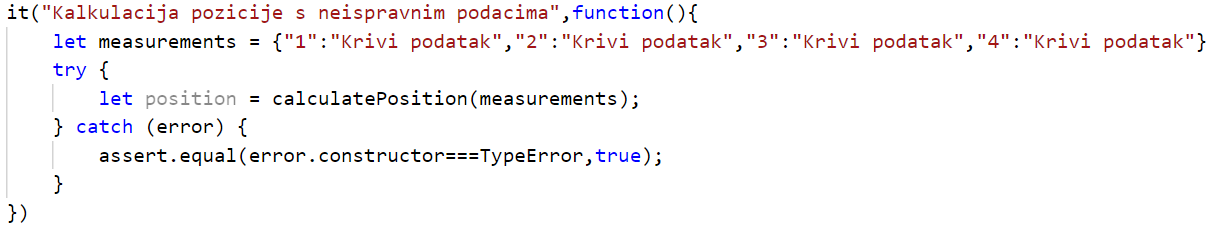
\includegraphics[width=1\linewidth]{"slike/kalkulacijaSNeispravnimPodacima.png"}
					\caption{Kalkulacija s neispravnim podacima}
					\label{fig:neisp-kal}
				\end{figure}


			% TODO: \usepackage{graphicx} required
				\begin{figure}[H]
					\centering
					
\includegraphics[width=1\linewidth]{"slike/rezultati.png"}
					\caption{Prikaz rezultata izvođenja JUnit testova u razvojnom okruženju}
					\label{fig:rez}
				\end{figure}
			
			\eject
			\subsection{Ispitivanje sustava}
			
			{Ispitivanje je provedeno pomoću Selenium IDE. Cilj je bila provjera funkcionalnosti, rubnih uvjeta i pogrešaka u sustavu. Selenium IDE je potrebno instalirati kao ekstenziju u tražilici. Zatim, nakon postavljanja URL-a testirane stranice, izvrši se test čije akcije ostaju pamćene u okviru Seleniuma i kako bi se test mogao izvršavati automatiziriano. Testovi su izvršeni na aplikaciji otvorenoj na lokalnom računalu. \hfill\break


{\noindent \textbf{\textit{Ispitni slučaj 1: Registracija}}\\
\textbf{Uvjeti}:
			 \begin{enumerate}
				\item Prilikom pokretanja testa korisnik ne smije već biti prijavljen.
				\item Korisnik mora otvoriti stranicu za registraciju na PassDirect-u.
			 \end{enumerate}
\textbf{Očekivani rezultat}: Registracija neće uspijeti za netočno potvrđenu lozinku i netočan oblik e-maila, a uspjet će ako se točno ispravi i pokuša ponovno.\\
\textbf{Tijek}:
			 \begin{enumerate}
			 	\item U polja na registracijskom obrascu uneseni su korisnički podatci s krivom potvrdom lozinke i krivim formatom e-maila.
			 	\item Odabir gumba za registraciju.
			 	\item Ispis poruke i odbijanje registracije zbog neispravnih podataka.
			 	\item Točno ispravljena potvrda lozinke.
			 	\item Ispis poruke i odbijanje registracije zbog neispravnih podataka.
			 	\item Točno ispravljen e-mail.
			 	\item Odabir gumba za registraciju.
			 	\item Prihvat registracije i prikaz početnog ekrana.
			 \end{enumerate}
			 \noindent \textbf{Rezultat}:
			 Svi očekivani rezultati su zadovoljeni. Aplikacija je prošla test. \\

\begin{lstlisting}
Running 'Registracija'
open on /login OK
click on css=.register OK
click on name=firstname OK
type on name=firstname with value Ivan OK
type on name=lastname with value Ivanic OK
type on name=email with value kriviemail@email@email.com OK
type on name=password with value Lozinka123 OK
type on name=confirmpassword with value KrivaLozinka OK
sendKeys on name=confirmpassword with value ${KEY_ENTER} OK
click on css=.app-wrapper OK
type on name=confirmpassword with value Lozinka123 OK
sendKeys on name=confirmpassword with value ${KEY_ENTER} OK
mouseDownAt on css=.app-wrapper with value 24,368 OK
mouseMoveAt on css=.app-wrapper with value 24,368 OK
mouseUpAt on css=.app-wrapper with value 24,368 OK
click on css=.app-wrapper OK
type on name=email with value dobaremail@email.com OK
sendKeys on name=email with value ${KEY_ENTER} OK
'Registracija' completed successfully
\end{lstlisting}}\hfill\break





{\noindent \textbf{\textit{Ispitni slučaj 2: Neispravna prijava}}\\
\textbf{Uvjeti}:
			 \begin{enumerate}
				\item Prilikom pokretanja testa korisnik ne smije već biti prijavljen.
				\item Korisnik mora otvoriti početnu stranicu PassDirecta(Login).
			 \end{enumerate}
\textbf{Očekivani rezultat}: Prijava u stranicu će biti odbijena zbog unosa e-maila neregistriranog korisnika.\\
\textbf{Tijek}:
			 \begin{enumerate}
			 	\item U polja na obrascu za prijavu uneseni su e-mail za koji ne postoji prijavljeni korisnik u sustavu i lozinka.
			 	\item Odabir gumba za registraciju.
			 	\item Ispis poruke i odbijanje prijave zbog neispravnih podataka.
			 \end{enumerate}
			 \noindent \textbf{Rezultat}:
			 Očekivani rezultat je zadovoljen, pošto korisnik nije ulogiran. Aplikacija je prošla test. \\


\begin{lstlisting}
Running 'Neispravna prijava'
open on /login OK
click on name=email OK
type on name=email with value kriviEmail@email.com OK
type on name=password with value Lozinka123 OK
click on css=.submit OK
mouseOver on css=.submit OK
mouseOut on css=.submit OK
'Neispravna prijava' completed successfully
\end{lstlisting}}\hfill\break





{\noindent \textbf{\textit{Ispitni slučaj 3: Prijava, pretraga voznog reda i kupnja karte}}\\
\textbf{Uvjeti}:
			 \begin{enumerate}
				\item Prilikom pokretanja testa korisnik ne smije već biti prijavljen.
				\item Korisnik mora otvoriti početnu stranicu PassDirecta(Login).
			 \end{enumerate}
\textbf{Očekivani rezultat}: Uspješna prijava u stranicu PassDirecta, pretraga voznog reda, te kupnja karte za odabranu liniju, odnosno vlak.\\
\textbf{Tijek}:
			 \begin{enumerate}
			 	\item U polja na obrascu za prijavu uneseni su e-mail i lozinka za postojećeg korisnika.
			 	\item Odabir gumba za registraciju.
			 	\item Prikaz početnog ekrana aplikacije.
				\item Odabir mjesta polaska i mjesta dolaska te datuma putovanja u zaglavlju stranice.
				\item Odabir gumba za pretraživanje voznog reda.
				\item Prikaz dostupnih linija za odabrane podatke.
				\item Odabir željene linije za koju se kupuje karta.
				\item Prikaz ekrana za checkout s već popunjenim e-mailom, imenom i prezimenom.
				\item Unos podataka o kartici.
				\item Odabir gumba za plaćanje.
				\item Prikaz obavijesti o uspješnoj transakciji.
			 \end{enumerate}
			 \noindent \textbf{Rezultat}:
			 Očekivani rezultati se zadovoljeni: nakon prijave u sustav, korisnik pretraži vozni red i kupi kartu. Aplikacija je prošla test. \\




\begin{lstlisting}
Running 'Prijava, pretraga voznog reda i kupnja karte'
open on /login OK
click on name=email OK
type on name=email with value pero@email.com OK
type on name=password with value Lozinka123 OK
sendKeys on name=password with value ${KEY_ENTER} OK
click on name=to OK
select on name=to with value label=Split OK
click on css=.right > .button OK
mouseOver on css=.right > .button OK
mouseOut on css=.right > .button OK
click on xpath=//div[@id='100']/h5/span[8]/button OK
click on id=cardNo OK
type on id=cardNo with value 1111 1111 1111 1111 OK
click on id=CVV OK
type on id=CVV with value 111 OK
click on id=expDate OK
click on id=expDate OK
click on id=expDate OK
type on id=expDate with value 0001-01 OK
type on id=expDate with value 0012-01 OK
click on css=.submit OK
click on css=.button-succesful OK
'Kupnja karte' completed successfully
\end{lstlisting}}\hfill\break






{\textbf{\textit{Ispitni slučaj 4: Prijava administratora, ispis korisnika i brisanje korisnika}}\\
\textbf{Uvjeti}:
			 \begin{enumerate}
				\item Prilikom pokretanja testa korisnik ne smije već biti prijavljen.
				\item Korisnik mora otvoriti početnu stranicu PassDirecta(Login).
				\item Korisnik prije prijave mora imati dodijeljenu rolu administratora.
				\item U bazi/sustavu mora postojati barem jedan korisnik koji.
			 \end{enumerate}
\textbf{Očekivani rezultat}: Uspješna prijava administratora u stranicu, pregled ispisa korisnika i brisanje korisničkih profila.\\
\textbf{Tijek}:
			 \begin{enumerate}
			 	\item U polja na obrascu za prijavu uneseni su e-mail i lozinka za postojećeg administratora.
			 	\item Odabir gumba za registraciju.
			 	\item Prikaz početnog ekrana aplikacije s listom korisnika.
				\item Odabir gumba za brisanje kraj jednog od korisnika.
				\item Korisnik je obrisan iz baze podataka.
				\item Prikaz osvježene liste korisnika.
			 \end{enumerate}
			 \noindent \textbf{Rezultat}:
			 Očekivani rezultati se zadovoljeni: nakon prijave u sustav, administrator pregleda i izbriše korisnika. Aplikacija je prošla test. \\



\begin{lstlisting}
Running 'Prijava administratora,ispis korisnika i brisanje profila'
open on /login OK
click on name=email OK
type on name=email with value admin@email.com OK
type on name=password with value Lozinka123 OK
sendKeys on name=password with value ${KEY_ENTER} OK
click on css=#korisnik1\@email\.com span:nth-child(5) > .buttonAH OK
'Prijava administratora,ispis korisnika i brisanje profila' completed 
successfully
\end{lstlisting}
 }}
	
 
 
	
			
			\eject 
		
		
		\section{Dijagram razmještaja}
			
			{Dijagram razmještaja statički opisuje topologiju sustava s fokusom na odnos skopovlja i programskog dijela projekta. Organizacija sustava se zasniva na arhitekturi klijent - poslužitelj. Klijent na svome računalu koristi web preglednik kako bi pristupio aplikaciji koja se nalazi na Heroku servisu. Više korisnika može pristupiti aplikaciji, putem HTTP veze. Heroku web server sadrži web poslužitelj i poslužitelj baze podataka na kojima se nalaze sama aplikacija, odnosno baza podataka aplikacije. }
				
			 % TODO: \usepackage{graphicx} required
				\begin{figure}[H]
					\centering
					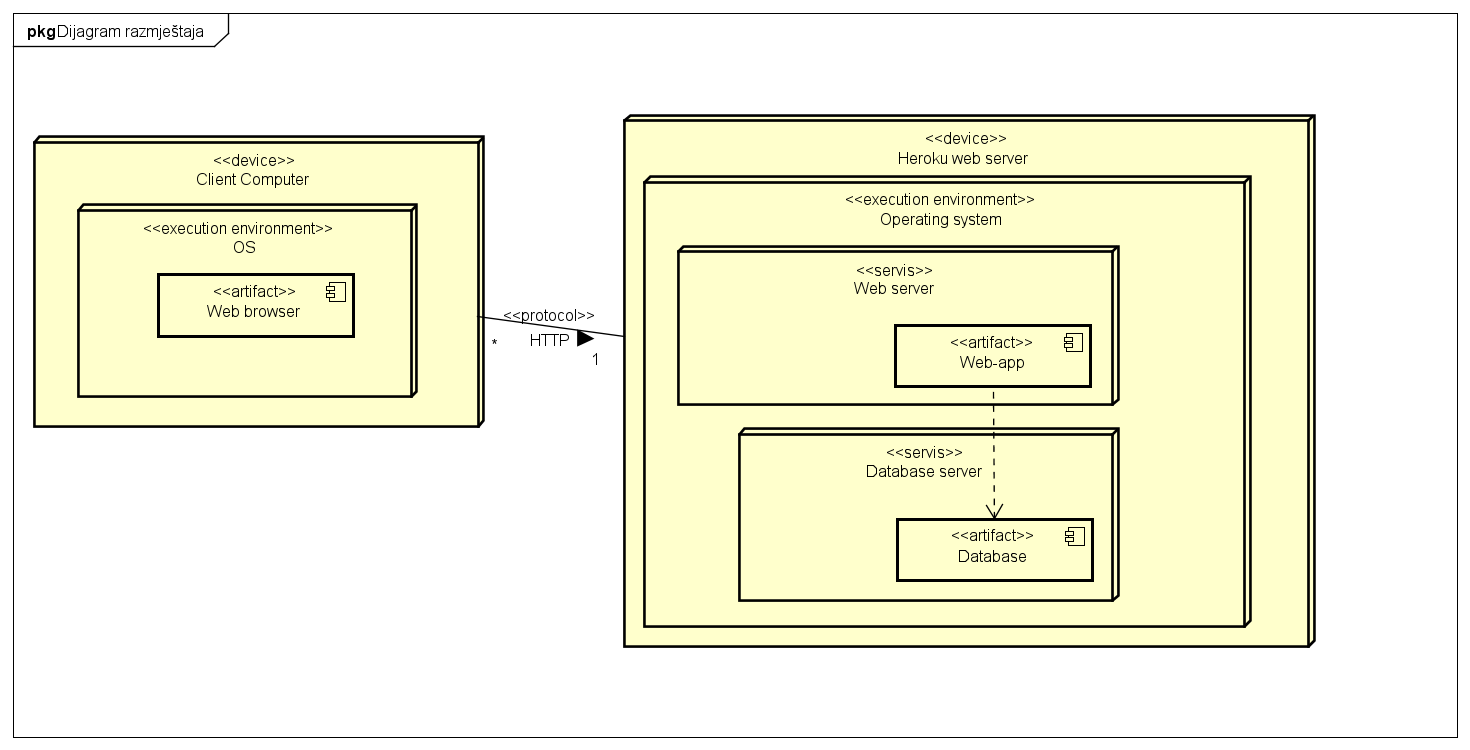
\includegraphics[width=1\linewidth]{"slike/specDiagram.png"}
					\caption{Dijagram razmještaja}
					\label{fig:dij-raz}
				\end{figure}
			
			\eject 
		
		\section{Upute za puštanje u pogon}
		
			 {U ovom poglavlju opisano je puštanje aplikacije u pogon. Puštanje je izvedeno uz pomoć platforme Heroku. 
%TODO: \usepackage{graphicx} required
				\begin{figure}[H]
					\centering
					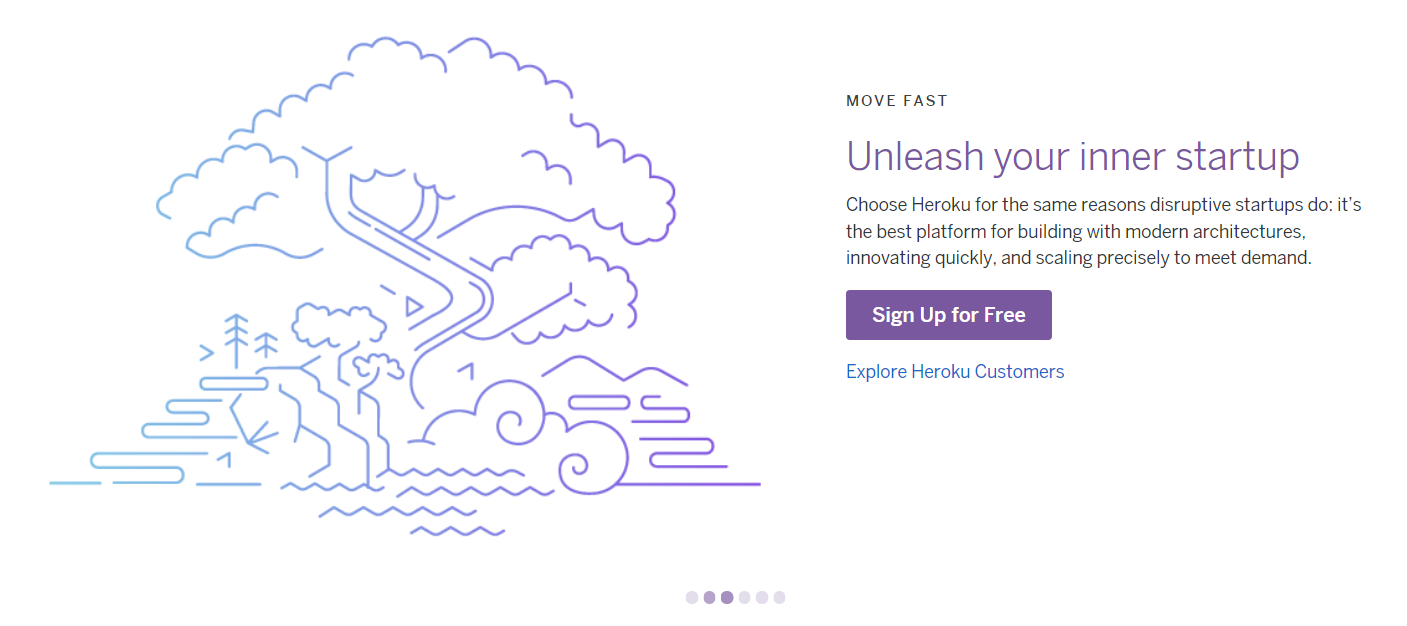
\includegraphics[width=1\linewidth]{"slike/herokuPocetna.png"}
					\caption{Platforma Heroku}
				\end{figure}
			
			
Najprije je potrebno registrirati račun te se prijaviti. Nakon prijave korisniku je otvorena stranica sa postojećim aplikacijama te opcijom za stvaranje nove. 
%TODO: \usepackage{graphicx} required
				\begin{figure}[H]
					\centering
					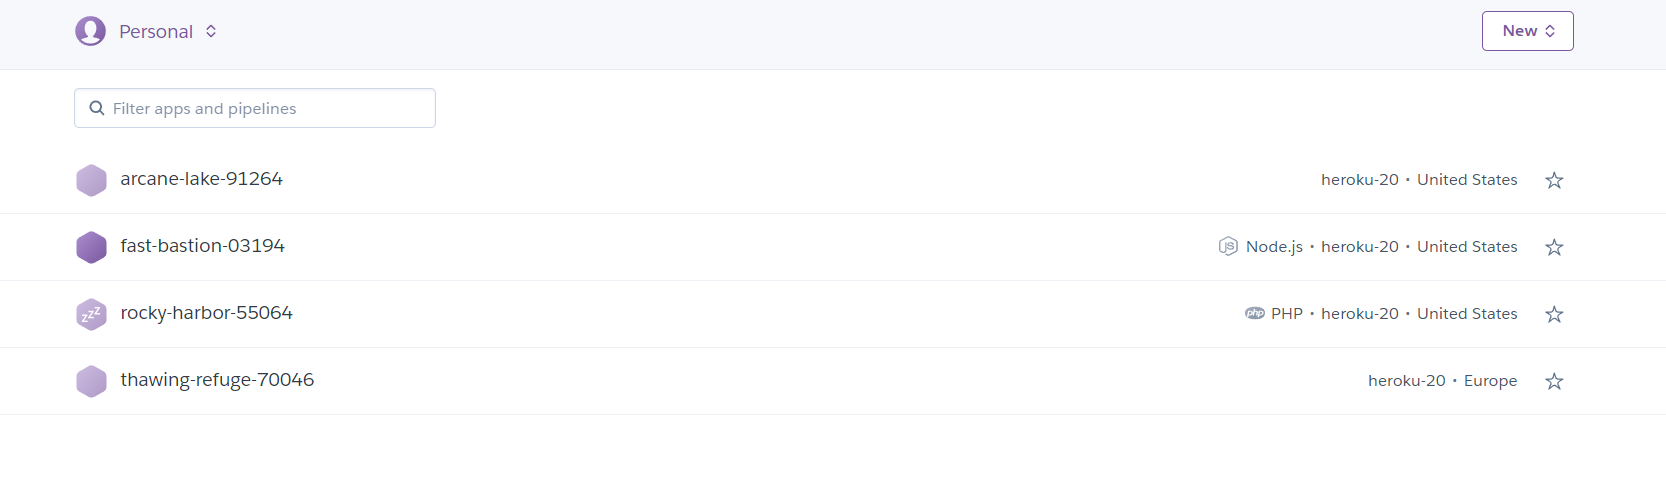
\includegraphics[width=1\linewidth]{"slike/herokuNewApp.png"}
					\caption{1. korak: "New"}
				\end{figure}
\eject			
			
 Odabirom gumba za stvaranje nove aplikacije otvara se obrazac za popunjavanje polja za osnovne informacije o aplikaciji (naziv i regija).
%TODO: \usepackage{graphicx} required
				\begin{figure}[H]
					\centering
					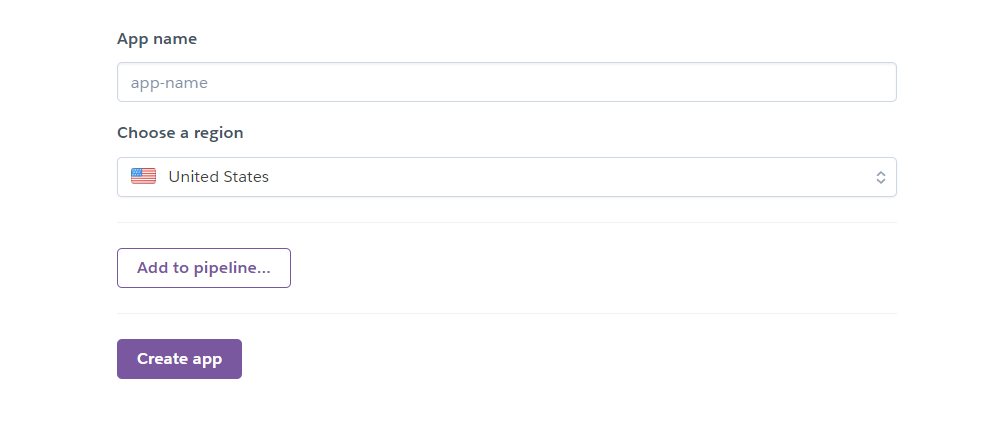
\includegraphics[width=1\linewidth]{"slike/herokuNew.png"}
					\caption{2. korak: Obrazac}
				\end{figure}						
			
Nakon što su je Heroku platformi napravljena i postavljena aplikacija, još je preostao upload izvornog koda uz pomoć HerokuCLI. U terminalu na računalu se pozicionira u direktorij IzvorniKod i unese se naredba za login u heroku:
\newline - heroku login \newline
Sada moramo izvesti sljedeće naredbe kako bismo postavili aplikaciju na Heroku:
\newline  - cd ../izvorniKod 
\newline - heroku git: remote -a naziv-aplikacije-na-heroku
\newline - git add .
\newline - git commit -m "Commit"
\newline - git push heroku master \newline
\textbf{Kreiranje baze podataka}\\
{U ormconfig.json datoteci su nam zapisani podaci za povezivanje i kreiranje baze podataka kako je prikazano na slici ispod. 
%TODO: \usepackage{graphicx} required
				\begin{figure}[H]
					\centering
					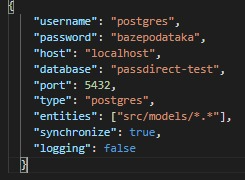
\includegraphics[width=0.6\linewidth]{"slike/inicijalizacijaBP.png"}
					\caption{Kreiranje baze podataka}
				\end{figure}			
Kako bismo imali kontrolu nad našom bazom podataka koja se sada nalazi na herokuovom serveru, za naš heroku projekt dodajemo Heroku Postgres plugin. Ovaj plugin nam omogućuje da se premjestimo u psql CLI te otud koristeći SQL upite kontroliramo i izmjenjujemo stanje BP. Kako bismo pokrenuli CLI potrebno je u terminalu računala na kojem radimo upisati naredbu: heroku pg:psql --app pass-direct
}		
}
			
			
			
			\eject 
	\chapter{Zaključak i budući rad}

		{Zadatak naše projektne grupe bio je razvoj aplikacije za pregled i kupnju karata za vlakove s ciljem očuvanja željezničke infrastrukture prijevoznika. Nakon nešto više od 3 mjeseca rada, uglavnom smo uspjeli ostvariti taj cilj. Naš projekt se odvijao u dvama ciklusima. }

		{U prvome ciklusu, na početku samoga projekta najveći problemi bili su neiskustvo većine članova s alatima potrebnim za izradu aplikacije te grupni rad na ovakvom tipu zadatka (projekta), no vremenom se stekao osjećaj za rad u timu i radom su se stekla nova znanja i vještine s dotad nepoznatom programskom podrškom. Nakon odabira vođe projekta i okvirne podijele posla, izradili su se obrasci uporabe i njima pripadajući dijagrami koji su uvelike pomogli pri početku razvoja aplikacije kao glavne vodilje pri nastalim nejasnoćama i nedoumicama. Cilj prvoga ciklusa je bio da se napravi kostur aplikacije i osnovne funkcionalnosti koje će se u drugom ciklusu nadograditi i specifirati. }

		{U drugome ciklusu tim je podijeljen na \textit{backend} i \textit{frontend} timove zbog lakšeg i efikasnijeg rada. Dokumentacija je dorađena nakon prvog kolokviranja te se dalje izrađivala postupno s gradivom. Izrada i promjena aplikacije morala je biti u skladu s njom, što je u trenutcima bilo dosta korisno. U ovome ciklusu se pokazao odličan timski rad, unatoč tome što se većina članova tima morala upoznavati s novim alatima i metodama rada. Velik se dio funkcionalnosti napravio u ovom ciklusu uz intenzivan, ali efikasan rad.}

		{Komunikacija je tekla putem WhatsApp-a što je pospiješilo informiranost i brzo riješavanje problema. Komunikacija je vremenom postajala sve bolja i opuštenija, što je dobro utjecalo na uspjehe tima. }

		{Rad na ovome projektu bio je cijelome timu odlično iskustvo za daljnji rad u timovima, a iskustvo s novim tehnologijama i alatima može samo pomoći individualnim inženjerskim razvojima. Svijesni smo da su neke stvari mogle ići lakše, bolje, drugačije i efikasnije, ali smo na koncu zadovoljni rezultatom i sigurni smo da ćemo iz ovog projekta izvući puno dobrih stvari. }
		
		\eject 
	\chapter*{Popis literature}
		\addcontentsline{toc}{chapter}{Popis literature}
	 	
		
		\begin{enumerate}
			
			
			\item  Programsko inženjerstvo, FER ZEMRIS, \url{http://www.fer.hr/predmet/proinz}
			
			\item  The Unified Modeling Language, \url{https://www.uml-diagrams.org/}
			
			\item  Astah Community, \url{http://astah.net/editions/uml-new}
			
			\item Software design-Vlado Sruk,
			
			\url {https://moodle.fer.hr/pluginfile.php/78699/mod_resource/content/1/erasmus_Software%20Design..pdf}
			
			\item Git community, \url{http://git-scm.com/}
			
			\item Gitlab Platform,\url{https://about.gitlab.com/}
			
			\item ReactJs community,  \url{https://reactjs.org/docs/getting-started.html}
			
			\item Express, \url{https://expressjs.com/}
			
			\item Typescript community, \url{https://www.typescriptlang.org/}
			
			\item pgAdmin organization, \url{https://www.pgadmin.org/}
			
			\item Use Case Modeling, \url{https://books.google.hr/books?id=zvxfXvEcQjUC&printsec=frontcover&dq=Use+Case+Modeling:+Software+Systems&hl=hr&sa=X&ved=0ahUKEwijxbTF0p3lAhWGbFAKHeuFC_gQ6AEIMTAB#v=onepage&q=Use%20Case%20Modeling%3A%20Software%20Systems&f=false}
			
			\item Git visualization, \url{http://git-school.github.io/visualizing-git/#free}
			
			\item W3Schools, \url{https://www.w3schools.com/}

			\item HŽ putnički prijevoz, \url{http://www.hzpp.hr/}

			\item Citymapper, \url{https://citymapper.com/}
			
		\end{enumerate}
		
		 

	\begingroup
	\renewcommand*\listfigurename{Indeks slika i dijagrama}
	%\renewcommand*\listtablename{Indeks tablica}
	%\let\clearpage\relax
	\listoffigures
	%\vspace{10mm}
	%\listoftables
	\endgroup
	\addcontentsline{toc}{chapter}{Indeks slika i dijagrama}

	\eject

	\chapter*{Dodatak: Prikaz aktivnosti grupe}
		\addcontentsline{toc}{chapter}{Dodatak: Prikaz aktivnosti grupe}
		
		\section*{Dnevnik sastajanja}
		
		
		\begin{packed_enum}
			\item  sastanak
			
			\item[] \begin{packed_item}
				\item Datum: 07.10.2021.
				\item Prisustvovali: T. Pavković, M. Vučinić, A. Vinković, K. Pavlović, F. Cindrić, M. Galić, I. Hajpek
				\item Teme sastanka:
				\begin{packed_item}
					\item  Razgovor o poznavanju tehnologija
					\item  Dogovor o tutorialima i upute za okviran način rad
				\end{packed_item}
			\end{packed_item}
			
			\item  sastanak
			\item[] \begin{packed_item}
				\item Datum: 16.10.2021.
				\item Prisustvovali: T. Pavković, M. Vučinić, A. Vinković, K. Pavlović, F. Cindrić, M. Galić, I. Hajpek
				\item Teme sastanka:
				\begin{packed_item}
					\item  Komentiranje dobivene teme i razjašnjavanje nejasnoća
					\item  Upoznavanje s GitLab-om i LaTex-om
				\end{packed_item}
			\end{packed_item}

			\item  sastanak
			\item[] \begin{packed_item}
				\item Datum: 23.10.2021.
				\item Prisustvovali: T. Pavković, M. Vučinić, A. Vinković, K. Pavlović, F. Cindrić, M. Galić, I. Hajpek
				\item Teme sastanka:
				\begin{packed_item}
					\item  Dogovorene razvojne okoline i tehnologije
					\item  Rasprava o izradi generičkih sposobnosti
					\item  Dogovor za početak razvijanje aplikacija
					\item  Dogovoren početak rada na predlošku dokumentacije i izgledu stranice
				\end{packed_item}
			\end{packed_item}

			
			\item  sastanak
			\item[] \begin{packed_item}
				\item Datum: 30.10.2021.
				\item Prisustvovali: T. Pavković, M. Vučinić, A. Vinković, K. Pavlović, F. Cindrić, M. Galić, I. Hajpek
				\item Teme sastanka:
				\begin{packed_item}
					\item  Pregled prethodno zadanih zadataka
					\item  Određen kostur aplikacije
					\item  Završene početne verzije UC-ova i dijagrama
					\item  Početak dizajna baze podataka
				\end{packed_item}
			\end{packed_item}

			
			\item  sastanak
			\item[] \begin{packed_item}
				\item Datum: 06.11.2021.
				\item Prisustvovali: T. Pavković, M. Vučinić, A. Vinković, K. Pavlović, F. Cindrić, M. Galić, I. Hajpek
				\item Teme sastanka:
				\begin{packed_item}
					\item  Dorađivanje dokumentacije
					\item  Modeliranje entiteta i dizajn kontrolera
					\item  Dorađivanje dosadašnjeg front-end-a
				\end{packed_item}
			\end{packed_item}

			
			\item  sastanak
			\item[] \begin{packed_item}
				\item Datum: 14.11.2021.
				\item Prisustvovali: T. Pavković, M. Vučinić, A. Vinković, K. Pavlović, F. Cindrić, M. Galić, I. Hajpek
				\item Teme sastanka:
				\begin{packed_item}
					\item  Provjere na front-endu
					\item  Pravljenje arhitekture i dizajna sustava u dokumentaciji
					\item  Daljnji rad na back-endu, kontrolerima i modelima
				\end{packed_item}
			\end{packed_item}

			
			\item  sastanak
			\item[] \begin{packed_item}
				\item Datum: 16.11.2021.
				\item Prisustvovali: T. Pavković, M. Vučinić, A. Vinković, K. Pavlović, F. Cindrić, M. Galić, I. Hajpek
				\item Teme sastanka:
				\begin{packed_item}
					\item  Završne promjene na dokumentaciji i bazi podataka
					\item  Povezivanje back-enda i front-enda
					\item  Dizanje baze na Heroku i deployanje aplikacije
				\end{packed_item}
			\end{packed_item}

			\item  sastanak
			\item[] \begin{packed_item}
				\item Datum: 6.12.2021.
				\item Prisustvovali: T. Pavković, M. Vučinić, A. Vinković, K. Pavlović, F. Cindrić, M. Galić, I. Hajpek
				\item Teme sastanka:
				\begin{packed_item}
					\item  Napravljen pregled programske podrške projekta
					\item  Podijela projektnog tima na backend i frontend
					\item  Frontend: fokus na radu funkcionalnog prikaza voznog reda i kupnje karata
					\item  Backend: uređivanje ruta i rad na kontrolerima 
				\end{packed_item}
			\end{packed_item}

			\item  sastanak
			\item[] \begin{packed_item}
				\item Datum: 14.12.2021.
				\item Prisustvovali: T. Pavković, M. Vučinić, A. Vinković, K. Pavlović, F. Cindrić, M. Galić, I. Hajpek
				\item Teme sastanka:
				\begin{packed_item}
					\item  Napravljen pregled odrađenih poslova s prošlog sastanka
					\item  Povezivanje frontenda i backenda
					\item  Dorađivanje Admin stranica na frontendu
					\item  Rad na implementaciji senzora
					\item  Nastavak rada na UML dijagramima
				\end{packed_item}
			\end{packed_item}

			\item  sastanak
			\item[] \begin{packed_item}
				\item Datum: 18.12.2021.
				\item Prisustvovali: T. Pavković, M. Vučinić, A. Vinković, K. Pavlović, F. Cindrić, M. Galić, I. Hajpek
				\item Teme sastanka:
				\begin{packed_item}
					\item  Privođenje kraju posla na frontendu, dorađivanje izgleda
					\item  Rad na implementaciji kontrolera za senzore i načinu dohvata podataka senzora
					\item  Rad na dokumentaciji postupno s gradivom
					\item  Provjera konzistentnosti i uređivanje modela na backendu
				\end{packed_item}
			\end{packed_item}

			\item  sastanak
			\item[] \begin{packed_item}
				\item Datum: 12.1.2022.
				\item Prisustvovali: T. Pavković, M. Vučinić, A. Vinković, K. Pavlović, F. Cindrić, M. Galić, I. Hajpek
				\item Teme sastanka:
				\begin{packed_item}
					\item  Dorađivanje pojedinosti vezanih uz senzore
					\item  Unit testing
					\item  Izrada podataka za punjenje baze podataka
					\item  Provjera i testiranje rada aplikacije
				\end{packed_item}
			\end{packed_item}
			
			%
			
		\end{packed_enum}
		
		\eject
		\section*{Tablica aktivnosti}
		
			
		

			\begin{longtblr}[
					label=none,
				]{
					vlines,hlines,
					width = \textwidth,
					colspec={X[7, l]X[1, c]X[1, c]X[1, c]X[1, c]X[1, c]X[1, c]X[1, c]}, 
					vline{1} = {1}{text=\clap{}},
					hline{1} = {1}{text=\clap{}},
					rowhead = 1,
				} 
				\multicolumn{1}{c|}{} & \multicolumn{1}{c|}{\rotatebox{90}{\textbf{Tomislav Pavković}}} & \multicolumn{1}{c|}{\rotatebox{90}{\textbf{Ante Vinković }}} &	\multicolumn{1}{c|}{\rotatebox{90}{\textbf{Martina Galić }}} & \multicolumn{1}{c|}{\rotatebox{90}{\textbf{Filip Cindrić }}} &	\multicolumn{1}{c|}{\rotatebox{90}{\textbf{Krešimir Pavlović }}} & \multicolumn{1}{c|}{\rotatebox{90}{\textbf{Mirta Vučinić }}} &	\multicolumn{1}{c|}{\rotatebox{90}{\textbf{Ivan Hajpek }}} \\  
				Upravljanje projektom 		& 15 & 3 &  &  &  &  & \\ 
				Opis projektnog zadatka 	&  &  & 7  &  & 3 & 1 & \\ 
				
				Funkcionalni zahtjevi       &  &  &  &  &  &  &  7  \\ 
				Opis pojedinih obrazaca 	&  &  &  &  & 2 &  & 9 \\ 
				Dijagram obrazaca 			&  &  & 5  &  & 1 &  & 1 \\ 
				Sekvencijski dijagrami 		&  &  & 7  &  &  &  & 4 \\ 
				Opis ostalih zahtjeva 		&  &  &  &  &  &  & 3 \\ 

				Arhitektura i dizajn sustava	 & 1 & 2 & 5 &  & 2 &  & 4 \\ 
				Baza podataka				&  & 3 & 14 &  &  &  &  11 \\ 
				Dijagram razreda 			&  &  & 6 &  &  &  & 6  \\ 
				Dijagram stanja				&  &  &  &  & 3 &  &  \\ 
				Dijagram aktivnosti 		&  &  &  &  &  &  & 3 \\ 
				Dijagram komponenti			&  &  &  &  & 3 &  &  \\ 
				Korištene tehnologije i alati 		&  & 1 &  &  &  &  & 2 \\ 
				Ispitivanje programskog rješenja 	&  &  &  &  & 15 &  & 10 \\ 
				Dijagram razmještaja			&  &  &  &  &  &  & 1 \\ 
				Upute za puštanje u pogon 		&  & 1 &  &  & 3 &  &  \\  
				Dnevnik sastajanja 			&  & 10 &  &  &  &  & 3 \\ 
				Zaključak i budući rad 		&  &  &  &  &  &  & 1 \\  
				Popis literature 			&  &  &  &  &  &  & 1 \\  

				\textit{Izrada početne stranice} 						& 8 &  &  &  & 15 & 6 & 1 \\  
				\textit{Izrada baze podataka} 		 				& 9 & 5 & 5 &  &  & 3 & \\  
				\textit{Spajanje s bazom podataka} 					& 10 & 8 &  &  &  & 25 &  \\ 
				\textit{Back end} 								& 55  & 20 & 17 &  &  &  &  \\  
				\textit{Login} 									& 5 &  &  &  & 5 & 12 &  \\  
				\textit{Registracija} 								& 7 &  &  &  &  & 15 &  \\  
				\textit{Admin home} 								& 6 &  &  & 16 &  & 8 & 2 \\  
				\textit{Pregled vlakova} 							& 15 &  & 8 &  &  & 7 & 3 \\  
				\textit{Kupnja karata} 							& 12 &  &  & 30 &  & 4 &  \\  
				\textit{Deploy}									& 4 & 5 & 5 &  &  &  & 5 \\  
				\textit{Izrada dizajna}								& 6 & 5 &  & 5 & 15 & 4 &  \\  
				\textit{Izrada testnih podataka}						&  & 15 &  & 2 &  &  &  \\
				\textit{Rad na senzorima}  							& 20 & 5 &  &  &  &  & \\ 
				\textit{Slanje mailova}							& 7 &  & 10 &  &  & 1 & \\ 
				\textit{Pregled transakcija}							&  &  &  & 5 &  &  & \\
 				\textit{Brisanje računa}							&  & 1 &  & 2 &  &  & \\
				\textit{Kalkulacija vagona i pozicija}					& 10 &  &  &  &  &  & \\
			\end{longtblr}
					
					
		\eject
		
		\section*{Dijagrami pregleda promjena}
		
		% TODO: \usepackage{graphicx} required
				\begin{figure}[H]
					\centering
					\includegraphics[width=0.6\linewidth]{"slike/developBranchActivity"}
					\caption{Dijagram aktivnosti na grani \textit{develop}}
					\label{fig:dijagram-dvlp}
				\end{figure}
				

		% TODO: \usepackage{graphicx} required
				\begin{figure}[H]
					\centering
					\includegraphics[width=0.75\linewidth]{"slike/devdocBranchActivity"}
					\caption{Dijagram aktivnosti na grani \textit{devdoc}}
					\label{fig:dijagram-doc}
				\end{figure}


\end{document}